% !Mode:: "TeX:UTF-8:Main"
% Source: https://davidcarlisle.github.io/latexcgi/test2#scottish-play
% LaTeX markup from limpidsoft. http://www.limpidsoft.com/plays/
% adapted to allow tagging

\DocumentMetadata{
 lang=en,
 pdfversion=2.0,
 pdfstandard=ua-2,
 pdfstandard=a-4,
 testphase=
   {
    phase-III, %lists,footnotes,sectioning,
               %toc,marginpar,bibliography,floats,
               %graphics ...
    math,  
    table, %tabular, tabularx, longtable
    title  %maketitle
   }
 }


\documentclass{book}

%% specify the page size and margins. Here, we use A4 paper
\usepackage[a4paper,top=20mm,bottom=25mm,left=25mm,right=25mm]{geometry}
%		Typically, the margins will not be specified but, in this case, they are specified in 
%		order to minimise line wrapping in the content.
%		For reference, format for First Folio page size:
%		\usepackage[height=335mm,width=235mm,top=20mm,bottom=25mm,left=20mm,right=25mm]{geometry}

% specify the styles of the title and section headings
%UF:  TODO: do it without titlesec
%\usepackage[small,bf,it,sc,rm,center,compact]{titlesec}
%		the titles are specified to be small, bold, italic, small caps, roman, centered and compact.
%		try removing any or all of the parameters to alter the display.
\makeatletter
\def\@makechapterhead#1{%
  \vspace*{40\p@}%
  {\parindent \z@ \centering \timesfont\itshape
    \ifnum \c@secnumdepth >\m@ne
      \if@mainmatter
        \huge\bfseries \@chapapp\space \thechapter
        \par\nobreak
        \vskip 20\p@
      \fi
    \fi
    \interlinepenalty\@M
    \huge \bfseries #1\par\nobreak
    \vskip 40\p@
  }}

\renewcommand\section{\@startsection {section}{1}{\z@}%
                                   {-1ex \@plus -.5ex \@minus -.2ex}%
                                   {1ex \@plus.2ex}%
                                   {\centering\timesfont\large\bfseries\itshape\textsc}}

\makeatother
%% keep open the option of using balanced multicolumns:
\usepackage{multicol}

\usepackage{graphicx} % include graphics, as on our title page
\usepackage{fancyhdr} % fancy page headers: definitely the way to go

% Code for creating empty pages
% No headers on empty pages before new chapter see http://www.markschenk.com/tensegrity/latexexplanation.html
\makeatletter
\def\cleardoublepage{\clearpage\if@twoside \ifodd\c@page\else
    \hbox{}
    \thispagestyle{empty}
    \newpage
    \if@twocolumn\hbox{}\newpage\fi\fi\fi}
\makeatother \clearpage{\pagestyle{plain}\cleardoublepage}

% parindent allows us to control the appearance of text blocks.
% a positive value indents the first line, while a negative value outdents the first line,
% so that any wrapped lines appear indented. This is worth experimenting with.

% it is normally not necessary to specify the space between lines and between columns, but space is at a premium
% when setting out columns
 
\setlength\parindent{0em}% wrapped lines are aligned with the first line (try indenting them).
\setlength\parskip{2pt plus1pt minus1pt} % limit the space between paras (here, they are mostly single lines).
\setlength\columnsep{20mm} % setting for the body of the document

%% choice of standard fonts (font height and line height). You will not need all of these!
\ifx\directlua\undefined
\newcommand{\chanceryfont}{\fontsize{9}{10.5}\usefont{T1}{pzc}{m}{il}}
\newcommand{\avantgardefont}{\fontsize{9}{10.5}\usefont{T1}{pag}{m}{n}}
\newcommand{\helveticafont}{\fontsize{10}{11.5}\usefont{T1}{phv}{m}{n}}
\newcommand{\courierfont}{\fontsize{10}{11.5}\usefont{T1}{pcr}{m}{n}}
\newcommand{\timesfont}{\fontsize{10}{10.5}\usefont{T1}{ptm}{m}{n}}
\newcommand{\charterfont}{\fontsize{10}{11.5}\usefont{T1}{pch}{m}{n}}
\newcommand{\bookmanfont}{\fontsize{10}{11.5}\usefont{T1}{pbk}{m}{n}}
\newcommand{\palatinofont}{\fontsize{10}{11.5}\usefont{T1}{ppl}{m}{n}}
\else
\usepackage{fontspec}
\newfontfamily\utimesfont{TeX Gyre Termes}
\newcommand{\timesfont}{\fontsize{10}{10.5}\utimesfont}
\fi
\setcounter{secnumdepth}{-2} % suppress automatic numbering of headings: try commenting this out!

\newcommand{\HRule}{\noindent\rule{\linewidth}{1.5pt}} % rules on the title page.
\newcommand{\FRule}{\noindent\rule{\linewidth}{0.25pt}} % rules for section headings.

% The following are new definitions for styling a play, with Act/Scene headings and speeches
% that include: speaker, speech content, as well as inline and block stage directions.
% They are intended to interact and simplify the restyling of the final document.
% Note that most start with an uppercase letter to avoid clashes with standard LaTeX definitions.

%% Content blocks
\newcommand{\Act}[1]{\chapter{#1}}
\newcommand{\Scene}[1]{\FRule\section{#1}\vspace*{-1ex}\FRule\vspace*{2ex}}
\newcommand{\PgScene}[1]{\NewPage\FRule\section{#1}\vspace*{-1ex}\FRule\vspace*{2ex}}

%% Verse control
\newcommand{\Speaker}{\textsc } % speaker in small caps
\newcommand{\Spk}[1]{\Tab\Speaker{#1}} % full stop (period) after the speaker.
\newcommand{\Indent}[1]{\begin{quote}#1\end{quote}} 
\newcommand{\Tab}{\vspace*{1ex}\hspace*{-1.0em}}% negative indent gives outdent: used for the speaker line
\newcommand{\I}{\hspace*{1em}}
\newcommand{\V}{\vspace*{2ex}}

%% page header management
\newcommand{\HideHeaderLine}{\renewcommand\headrulewidth{0.0pt}}
\newcommand{\ShowHeaderLine}{\renewcommand\headrulewidth{0.4pt}}

%% line and block management
\newenvironment{indentpar}[1]
{\begin{list}{}%
  {\setlength{\leftmargin}{#1} \setlength{\rightmargin}{#1}} \item[]}
{\end{list}}

\newenvironment{smallquote}{\vspace*{-5ex}\begin{list}{}{\leftmargin=0.5em\rightmargin=2em}\item[]}{\end{list}}

\newcommand{\Gap}{{\vspace{0.5ex}}}% gap above a block
\newcommand{\Blk}[1]{\setlength\topsep{-0.5ex}\begin{trivlist}\item[]#1\end{trivlist}}% compact indented block: reduced space above and below and no indentation.
\newcommand{\sd}[1]{\emph{#1}}
% 		This is an inline emphasis string.
\newcommand{\ActSD}[1]{\begin{center}\large\textsc{#1}\end{center}}
%		This is an emphasis block for at the start of an Act, and not inside a Scene
%UF changed doenpe problem with grouping
\newcommand{\SD}[1]{%\setlength\topsep{-0.5ex}
\begin{trivlist}[beginsep=-0.5ex]\item[]\textit{#1}\end{trivlist}}
%		This is a compact italicised emphasis block: reduced space above and below and no indentation.
%UF avoid group
\newcommand{\IB}[1]{\begin{smallquote}\item[]#1\end{smallquote}}

\newcommand{\Sf}{\sffamily } % sansserif font: better than a typewriter font
%		Note that this is a declaration, and requires no braces (note the trailing space)

%		Hooks for page breaks: to simplify testing of final layout and hard page breaks
%\newcommand{\NewPage}{}% a dummy page break.
\newcommand{\NewPage}{\vfill\pagebreak}% use this definition to disable all page breaks.
\newcommand{\ForcePage}{\vfill\pagebreak}% a necessary page break without vfill
\newcommand{\NoPage}{}% no page break: to simplify testing of individual page breaks.
\newcommand{\Page}{\pagebreak}% a hook for a page break that can be redefined. Here, there is no vfill.

\newcommand{\Globals}{\timesfont\raggedright}
%		remove these declarations from the document body
\newcommand{\Columns}{\twocolumn}
%		beware: this declaration can trigger an unwanted page break

\usepackage[colorlinks, linkcolor=blue,pdftitle=The Tragedy Of Macbeth]{hyperref}

\begin{document}
\Globals %declare font and text alignment.
%times is a narrow font with minimal line wrapping, which is what we want here. Try palatinofont or charterfont!

\thispagestyle{empty} % no headers or footers
\pagenumbering{Roman} %to have unique package numbers
\HideHeaderLine
\vspace*{\stretch{2}}
\HRule
\begin{center}\Huge\itshape\bfseries \tagstructbegin{title=The Tragedy Of Macbeth}THE TRAGEDY OF MACBETH\tagstructend
\ (1606)\end{center}
\HRule

\vspace*{\stretch{5}}
\begin{center}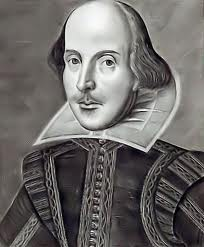
\includegraphics[scale=1,alt=William Shakespeare]{william-shakespeare.jpg}\end{center}
\vspace*{\stretch{5}}
\begin{center}\Large\bfseries by William Shakespeare\end{center}
\vspace*{\stretch{10}}

\begin{center}
\large Styled by LimpidSoft
\end{center}

\pagestyle{fancy}
\fancyhead{}
\NewPage\pagenumbering{roman}

% UF:  toc inside quote doesn't work
% UF TODO: adjust margin in some other way
% \begin{quote}\begin{quote}\tableofcontents\end{quote}\end{quote}
\tableofcontents
\NewPage

\begin{quote}\Sf\large

This text is an adaptation of part of the text supplied by Project Gutenberg [Etext \#100] and layout is in light of that in The Oxford Shakespeare (Clarendon Press, Oxford 1988).

Styling is broadly similar to that in the First Folio, particularly in the Scene headers. To improve readability, \textit{Speaker} lines are outdented, rather than indented, but this is easy to change in the document preamble.

The following is a part of the preamble to the Project Gutenberg Etext \#100:

\begin{quote}
This is the 100th Etext file presented by Project Gutenberg, and
is presented in cooperation with World Library, Inc., from their
Library of the Future and Shakespeare CDROMS.  Project Gutenberg
often releases Etexts that are NOT placed in the Public Domain!!

\hspace{5cm}  . . . . .

YOU MAY (AND ARE ENCOURAGED) TO DISTRIBUTE ELECTRONIC AND
MACHINE READABLE COPIES OF THIS ETEXT, SO LONG AS SUCH COPIES
(1) ARE FOR YOUR OR OTHERS PERSONAL USE ONLY, AND (2) ARE NOT
DISTRIBUTED OR USED COMMERCIALLY.  PROHIBITED COMMERCIAL
DISTRIBUTION INCLUDES BY ANY SERVICE THAT CHARGES FOR DOWNLOAD
TIME OR FOR MEMBERSHIP.

\hspace{5cm}  . . . . .

WRITE TO US! We can be reached at:\\
\I     Internet: hart@vmd.cso.uiuc.edu\\
\I\I       Bitnet: hart@uiucvmd\\
\I   CompuServe: >internet:hart@.vmd.cso.uiuc.edu\\
\I\I      Attmail: internet!vmd.cso.uiuc.edu!Hart\\
\I       Mail:  Prof. Michael Hart\\
\I\I               P.O. Box 2782\\
\I\I               Champaign, IL 61825
\end{quote}


Finally, note that this document is accompanied by the LaTeX text document that was used to generate it. Feel free to correct mistakes and improve/alter the format or style. Then use it to generate an improved, or reformatted, PDF document and pass it on to the world!


\begin{flushright}
John Redmond\\Sydney, Australia
\end{flushright}


\end{quote}


\ShowHeaderLine
\NewPage\pagenumbering{arabic}

\chapter{Dramatis Personae}

DUNCAN, King of Scotland

MACBETH, Thane of Glamis and Cawdor, a general in the King's army

LADY MACBETH, his wife

MACDUFF, Thane of Fife, a nobleman of Scotland

LADY MACDUFF, his wife

MALCOLM, elder son of Duncan

DONALBAIN, younger son of Duncan

BANQUO, Thane of Lochaber, a general in the King's army

FLEANCE, his son

LENNOX, nobleman of Scotland

ROSS, nobleman of Scotland

MENTEITH nobleman of Scotland

ANGUS, nobleman of Scotland

CAITHNESS, nobleman of Scotland

SIWARD, Earl of Northumberland, general of the English forces

YOUNG SIWARD, his son

SEYTON, attendant to Macbeth

HECATE, Queen of the Witches

The Three Witches

Boy, Son of Macduff

Gentlewoman attending on Lady Macbeth

An English Doctor

A Scottish Doctor

A Sergeant

A Porter

An Old Man

The Ghost of Banquo and other Apparitions

Lords, Gentlemen, Officers, Soldiers, Murtherers, Attendants, and Messengers


\Columns



\pagestyle{fancy}
\fancyhead{}
\fancyhead[L]{\leftmark}
\fancyhead[R]{\rightmark}

\Act{ACT I}

\ActSD{SCENE: Scotland and England}




\Scene{SCENE I}

\SD{A desert place. Thunder and lightning.\\
Enter three Witches}

\Spk{FIRST WITCH} When shall we three meet again?

In thunder, lightning, or in rain?

\Spk{SECOND WITCH} When the hurlyburly's done,

When the battle's lost and won.


\Spk{THIRD WITCH} That will be ere the set of sun

\Spk{FIRST WITCH} Where the place?

\Spk{SECOND WITCH} Upon the heath

\Spk{THIRD WITCH} There to meet with Macbeth

\Spk{FIRST WITCH} I come, Graymalkin

\Spk{ALL} Paddock calls

Fair is foul, and foul is fair.

Hover through the fog and filthy air. \sd{Exeunt}


\Scene{SCENE II}

\SD{A camp near Forres. Alarum within.\\
Enter Duncan, Malcolm, Donalbain, Lennox, with Attendants,
meeting a bleeding Sergeant}

\Spk{DUNCAN} What bloody man is that? He can report,

As seemeth by his plight, of the revolt

The newest state.

\Spk{MALCOLM} This is the sergeant

Who like a good and hardy soldier fought

'Gainst my captivity. Hail, brave friend!

Say to the King the knowledge of the broil

As thou didst leave it.

\Spk{SERGEANT} Doubtful it stood,

As two spent swimmers that do cling together

And choke their art. The merciless Macdonwald--

Worthy to be a rebel, for to that

The multiplying villainies of nature

Do swarm upon him--from the Western Isles

Of kerns and gallowglasses is supplied;

And Fortune, on his damned quarrel smiling,

Show'd like a rebel's whore. But all's too weak;

For brave Macbeth --well he deserves that name--

Disdaining Fortune, with his brandish'd steel,

Which smoked with bloody execution,

Like Valor's minion carved out his passage

Till he faced the slave,

Which ne'er shook hands, nor bade farewell to him,

Till he unseam'd him from the nave to the chaps,

And fix'd his head upon our battlements.

\Spk{DUNCAN} O valiant cousin! Worthy gentleman!

\Spk{SERGEANT} As whence the sun 'gins his reflection

Shipwrecking storms and direful thunders break,

So from that spring whence comfort seem'd to come

Discomfort swells. Mark, King of Scotland, mark.

No sooner justice had, with valor arm'd,

Compell'd these skipping kerns to trust their heels,

But the Norweyan lord, surveying vantage,

With furbish'd arms and new supplies of men,

Began a fresh assault.

\Spk{DUNCAN} Dismay'd not this

Our captains, Macbeth and Banquo.?

\Spk{SERGEANT} Yes,

As sparrows eagles, or the hare the lion.

If I say sooth, I must report they were

As cannons overcharged with double cracks,

So they

Doubly redoubled strokes upon the foe.

Except they meant to bathe in reeking wounds,

Or memorize another Golgotha,

I cannot tell--

But I am faint; my gashes cry for help.

\Spk{DUNCAN} So well thy words become thee as thy wounds;

They smack of honor both. Go get him surgeons.

\SD{Exit Sergeant, attended}

Who comes here?

\SD{Enter Ross}

\Spk{MALCOLM} The worthy Thane of Ross 

\Spk{LENNOX} What a haste looks through his eyes! So should he look

That seems to speak things strange.

\Spk{ROSS} God save the King!

\Spk{DUNCAN} Whence camest thou, worthy Thane?

\Spk{ROSS} From Fife, great King,

Where the Norweyan banners flout the sky

And fan our people cold.

Norway himself, with terrible numbers,

Assisted by that most disloyal traitor

The Thane of Cawdor, began a dismal conflict,

Till that Bellona's bridegroom, lapp'd in proof,

Confronted him with self-comparisons,

Point against point rebellious, arm 'gainst arm,

Curbing his lavish spirit; and, to conclude,

The victory fell on us.

\Spk{DUNCAN} Great happiness!

\Spk{ROSS} That now

Sweno, the Norways' king, craves composition;

Nor would we deign him burial of his men

Till he disbursed, at Saint Colme's Inch,

Ten thousand dollars to our general use.

\Spk{DUNCAN} No more that Thane of Cawdor shall deceive

Our bosom interest. Go pronounce his present death,

And with his former title greet Macbeth.

\Spk{ROSS} I'll see it done

\Spk{DUNCAN} What he hath lost, noble Macbeth hath won

\SD{Exeunt}

\Scene{SCENE III}

\SD{A heath. Thunder.\\
Enter the three Witches}

\Spk{FIRST WITCH} Where hast thou been, sister?

\Spk{SECOND WITCH} Killing swine

\Spk{THIRD WITCH} Sister, where thou?

\Spk{FIRST WITCH} A sailor's wife had chestnuts in her lap,

And mounch'd, and mounch'd, and mounch'd. "Give me," quoth I.

"Aroint thee, witch!" the rump-fed ronyon cries.

Her husband's to Aleppo gone, master the Tiger;

But in a sieve I'll thither sail,

And, like a rat without a tail,

I'll do, I'll do, and I'll do.

\Spk{SECOND WITCH} I'll give thee a wind

\Spk{FIRST WITCH} Thou'rt kind

\Spk{THIRD WITCH} And I another

\Spk{FIRST WITCH} I myself have all the other,

And the very ports they blow,

All the quarters that they know

I' the shipman's card.

I will drain him dry as hay:

Sleep shall neither night nor day

Hang upon his penthouse lid;

He shall live a man forbid.

Weary se'nnights nine times nine

Shall he dwindle, peak, and pine;

Though his bark cannot be lost,

Yet it shall be tempest-toss'd.

Look what I have.

\Spk{SECOND WITCH} Show me, show me

\Spk{FIRST WITCH} Here I have a pilot's thumb,

Wreck'd as homeward he did come. \sd{Drum within}

\Spk{THIRD WITCH} A drum, a drum!

Macbeth doth come.

\Spk{ALL} The weird sisters, hand in hand,

Posters of the sea and land,

Thus do go about, about,

Thrice to thine, and thrice to mine,

And thrice again, to make up nine.

Peace! The charm's wound up.

\SD{Enter Macbeth and Banquo}

\Spk{MACBETH} So foul and fair a day I have not seen

\Spk{BANQUO} How far is't call'd to Forres? What are these

So wither'd and so wild in their attire,

That look not like the inhabitants o' the earth,

And yet are on't? Live you? or are you aught

That man may question? You seem to understand me,

By each at once her choppy finger laying

Upon her skinny lips. You should be women,

And yet your beards forbid me to interpret

That you are so.

\Spk{MACBETH} Speak, if you can

\Spk{FIRST WITCH} All hail, Macbeth, hail to thee, Thane of Glamis!

\Spk{SECOND WITCH} All hail, Macbeth, hail to thee, Thane of Cawdor!

\Spk{THIRD WITCH} All hail, Macbeth, that shalt be King hereafter!

\Spk{BANQUO} Good sir, why do you start, and seem to fear

Things that do sound so fair? I' the name of truth,

Are ye fantastical or that indeed

Which outwardly ye show? My noble partner

You greet with present grace and great prediction

Of noble having and of royal hope,

That he seems rapt withal. To me you speak not.

If you can look into the seeds of time,

And say which grain will grow and which will not,

Speak then to me, who neither beg nor fear

Your favors nor your hate.

\Spk{FIRST WITCH} Hail!

\Spk{SECOND WITCH} Hail!

\Spk{THIRD WITCH} Hail!

\Spk{FIRST WITCH} Lesser than Macbeth, and greater

\Spk{SECOND WITCH} Not so happy, yet much happier

\Spk{THIRD WITCH} Thou shalt get kings, though thou be none

So all hail, Macbeth and Banquo!

\Spk{FIRST WITCH} Banquo and Macbeth, all hail!

\Spk{MACBETH} Stay, you imperfect speakers, tell me more

By Sinel's death I know I am Thane of Glamis;

But how of Cawdor? The Thane of Cawdor lives,

A prosperous gentleman; and to be King

Stands not within the prospect of belief,

No more than to be Cawdor. Say from whence

You owe this strange intelligence, or why

Upon this blasted heath you stop our way

With such prophetic greeting? Speak, I charge you.

\SD{Witches vanish}

\Spk{BANQUO} The earth hath bubbles as the water has,

And these are of them. Whither are they vanish'd?

\Spk{MACBETH} Into the air, and what seem'd corporal melted

As breath into the wind. Would they had stay'd!

\Spk{BANQUO} Were such things here as we do speak about?

Or have we eaten on the insane root

That takes the reason prisoner?

\Spk{MACBETH} Your children shall be kings

\Spk{BANQUO} You shall be King

\Spk{MACBETH} And Thane of Cawdor too

\Spk{BANQUO} To the selfsame tune and words

\SD{Enter Ross and Angus}

\Spk{ROSS} The King hath happily received, Macbeth,

The news of thy success; and when he reads

Thy personal venture in the rebels' fight,

His wonders and his praises do contend

Which should be thine or his. Silenced with that,

In viewing o'er the rest o' the selfsame day,

He finds thee in the stout Norweyan ranks,

Nothing afeard of what thyself didst make,

Strange images of death. As thick as hail

Came post with post, and every one did bear

Thy praises in his kingdom's great defense,

And pour'd them down before him.

\Spk{ANGUS} We are sent

To give thee, from our royal master, thanks;

Only to herald thee into his sight,

Not pay thee.

\Spk{ROSS} And for an earnest of a greater honor,

He bade me, from him, call thee Thane of Cawdor.

In which addition, hail, most worthy Thane,

For it is thine.

\Spk{BANQUO} What, can the devil speak true?

\Spk{MACBETH} The Thane of Cawdor lives

In borrow'd robes?

\Spk{ANGUS} Who was the Thane lives yet,

But under heavy judgement bears that life

Which he deserves to lose. Whether he was combined

With those of Norway, or did line the rebel

With hidden help and vantage, or that with both

He labor'd in his country's wreck, I know not;

But treasons capital, confess'd and proved,

Have overthrown him.

\Spk{MACBETH} \sd{Aside}

The greatest is behind. \sd{(To Ross and Angus)} Thanks for your pains.

\sd{(Aside to Banquo)} Do you not hope your children shall be kings,

When those that gave the Thane of Cawdor to me

Promised no less to them?

\Spk{BANQUO} \sd{Aside to Macbeth}

Might yet enkindle you unto the crown,

Besides the Thane of Cawdor. But 'tis strange;

And oftentimes, to win us to our harm,

The instruments of darkness tell us truths,

Win us with honest trifles, to betray's

In deepest consequence--

Cousins, a word, I pray you.

\Spk{MACBETH} \sd{Aside}

As happy prologues to the swelling act

Of the imperial theme--I thank you, gentlemen.

\sd{(Aside)} This supernatural soliciting

Cannot be ill, cannot be good. If ill,

Why hath it given me earnest of success,

Commencing in a truth? I am Thane of Cawdor.

If good, why do I yield to that suggestion

Whose horrid image doth unfix my hair

And make my seated heart knock at my ribs,

Against the use of nature? Present fears

Are less than horrible imaginings:

My thought, whose murther yet is but fantastical,

Shakes so my single state of man that function

Is smother'd in surmise, and nothing is

But what is not.

\Spk{BANQUO} Look, how our partner's rapt

\Spk{MACBETH} \sd{Aside}

Without my stir.

\Spk{BANQUO} New honors come upon him,

Like our strange garments, cleave not to their mould

But with the aid of use.

\Spk{MACBETH} \sd{Aside}

Time and the hour runs through the roughest day.

\Spk{BANQUO} Worthy Macbeth, we stay upon your leisure

\Spk{MACBETH} Give me your favor; my dull brain was wrought

With things forgotten. Kind gentlemen, your pains

Are register'd where every day I turn

The leaf to read them. Let us toward the King.

Think upon what hath chanced, and at more time,

The interim having weigh'd it, let us speak

Our free hearts each to other.

\Spk{BANQUO} Very gladly

\Spk{MACBETH} Till then, enough

\Scene{SCENE IV}

\SD{Forres. The palace.\\
Flourish. Enter Duncan, Malcolm, Donalbain, Lennox, and Attendants}

\Spk{DUNCAN} Is execution done on Cawdor? Are not

Those in commission yet return'd?

\Spk{MALCOLM} My liege,

They are not yet come back. But I have spoke

With one that saw him die, who did report

That very frankly he confess'd his treasons,

Implored your Highness' pardon, and set forth

A deep repentance. Nothing in his life

Became him like the leaving it; he died

As one that had been studied in his death,

To throw away the dearest thing he owed

As 'twere a careless trifle.

\Spk{DUNCAN} There's no art

To find the mind's construction in the face:

He was a gentleman on whom I built

An absolute trust.

\SD{Enter Macbeth, Banquo, Ross, and Angus}

O worthiest cousin!

The sin of my ingratitude even now

Was heavy on me. Thou art so far before,

That swiftest wing of recompense is slow

To overtake thee. Would thou hadst less deserved,

That the proportion both of thanks and payment

Might have been mine! Only I have left to say,

More is thy due than more than all can pay.

\Spk{MACBETH} The service and the loyalty lowe,

In doing it, pays itself. Your Highness' part

Is to receive our duties, and our duties

Are to your throne and state, children and servants,

Which do but what they should, by doing everything

Safe toward your love and honor.

\Spk{DUNCAN} Welcome hither

I have begun to plant thee, and will labor

To make thee full of growing. Noble Banquo,

That hast no less deserved, nor must be known

No less to have done so; let me infold thee

And hold thee to my heart.

\Spk{BANQUO} There if I grow,

The harvest is your own.

\Spk{DUNCAN} My plenteous joys,

Wanton in fullness, seek to hide themselves

In drops of sorrow. Sons, kinsmen, thanes,

And you whose places are the nearest, know

We will establish our estate upon

Our eldest, Malcolm, whom we name hereafter

The Prince of Cumberland; which honor must

Not unaccompanied invest him only,

But signs of nobleness, like stars, shall shine

On all deservers. From hence to Inverness,

And bind us further to you.

\Spk{MACBETH} The rest is labor, which is not used for you

I'll be myself the harbinger, and make joyful

The hearing of my wife with your approach;

So humbly take my leave.

\Spk{DUNCAN} My worthy Cawdor!

\Spk{MACBETH} \sd{Aside}

On which I must fall down, or else o'erleap,

For in my way it lies. Stars, hide your fires;

Let not light see my black and deep desires.

The eye wink at the hand; yet let that be

Which the eye fears, when it is done, to see. \sd{Exit}

\Spk{DUNCAN} True, worthy Banquo! He is full so valiant,

And in his commendations I am fed;

It is a banquet to me. Let's after him,

Whose care is gone before to bid us welcome.

It is a peerless kinsman. \sd{Flourish. Exeunt}

\Scene{SCENE V}

\SD{Inverness. Macbeth's castle.\\
Enter Lady Macbeth, reading a letter}

\Spk{LADY MACBETH} "They met me in the day of success, and I have
learned by the perfectest report they have more in them than
mortal knowledge. When I burned in desire to question them
further, they made themselves air, into which they vanished.

Whiles I stood rapt in the wonder of it, came missives from the
King, who all-hailed me 'Thane of Cawdor'; by which title,
before, these weird sisters saluted me and referred me to the
coming on of time with 'Hail, King that shalt be!' This have I
thought good to deliver thee, my dearest partner of greatness,
that thou mightst not lose the dues of rejoicing, by being
ignorant of what greatness is promised thee. Lay it to thy heart,
and farewell."

Glamis thou art, and Cawdor, and shalt be

What thou art promised. Yet do I fear thy nature.

It is too full o' the milk of human kindness

To catch the nearest way. Thou wouldst be great;

Art not without ambition, but without

The illness should attend it. What thou wouldst highly,

That wouldst thou holily; wouldst not play false,

And yet wouldst wrongly win. Thou'ldst have, great Glamis,

That which cries, "Thus thou must do, if thou have it;

And that which rather thou dost fear to do

Than wishest should be undone." Hie thee hither,

That I may pour my spirits in thine ear,

And chastise with the valor of my tongue

All that impedes thee from the golden round,

Which fate and metaphysical aid doth seem

To have thee crown'd withal.

\SD{Enter a Messenger}

What is your tidings?

\Spk{MESSENGER} The King comes here tonight

\Spk{LADY MACBETH} Thou'rt mad to say it!

Is not thy master with him? who, were't so,

Would have inform'd for preparation.

\Spk{MESSENGER} So please you, it is true; our Thane is coming

One of my fellows had the speed of him,

Who, almost dead for breath, had scarcely more

Than would make up his message.

\Spk{LADY MACBETH} Give him tending;

He brings great news. \sd{Exit Messenger}

The raven himself is hoarse

That croaks the fatal entrance of Duncan

Under my battlements. Come, you spirits

That tend on mortal thoughts, unsex me here

And fill me from the crown to the toe top-full

Of direst cruelty! Make thick my blood,

Stop up the access and passage to remorse,

That no compunctious visitings of nature

Shake my fell purpose nor keep peace between

The effect and it! Come to my woman's breasts,

And take my milk for gall, your murthering ministers,

Wherever in your sightless substances

You wait on nature's mischief! Come, thick night,

And pall thee in the dunnest smoke of hell

That my keen knife see not the wound it makes

Nor heaven peep through the blanket of the dark

To cry, "Hold, hold!"

\SD{Enter Macbeth}

Great Glamis! Worthy Cawdor!

Greater than both, by the all-hail hereafter!

Thy letters have transported me beyond

This ignorant present, and I feel now

The future in the instant.

\Spk{MACBETH} My dearest love,

Duncan comes here tonight.

\Spk{LADY MACBETH} And when goes hence?

\Spk{MACBETH} Tomorrow, as he purposes

\Spk{LADY MACBETH} O, never

Shall sun that morrow see!

Your face, my Thane, is as a book where men

May read strange matters. To beguile the time,

Look like the time; bear welcome in your eye,

Your hand, your tongue; look like the innocent flower,

But be the serpent under it. He that's coming

Must be provided for; and you shall put

This night's great business into my dispatch,

Which shall to all our nights and days to come

Give solely sovereign sway and masterdom.

\Spk{MACBETH} We will speak further

\Spk{LADY MACBETH} Only look up clear;

To alter favor ever is to fear.

Leave all the rest to me. \sd{Exeunt}

\Scene{SCENE VI}

\SD{Before Macbeth's castle.  Hautboys and torches.\\
Enter Duncan, Malcolm, Donalbain, Banquo, Lennox, Macduff, Ross, Angus,
and Attendants}

\Spk{DUNCAN} This castle hath a pleasant seat; the air

Nimbly and sweetly recommends itself

Unto our gentle senses.

\Spk{BANQUO} This guest of summer,

The temple-haunting martlet, does approve

By his loved mansionry that the heaven's breath

Smells wooingly here. No jutty, frieze,

Buttress, nor coign of vantage, but this bird

Hath made his pendant bed and procreant cradle;

Where they most breed and haunt, I have observed

The air is delicate.

\SD{Enter Lady Macbeth}

\Spk{DUNCAN} See, see, our honor'd hostess!

The love that follows us sometime is our trouble,

Which still we thank as love. Herein I teach you

How you shall bid God 'ield us for your pains,

And thank us for your trouble.

\Spk{LADY MACBETH} All our service

In every point twice done, and then done double,

Were poor and single business to contend

Against those honors deep and broad wherewith

Your Majesty loads our house. For those of old,

And the late dignities heap'd up to them,

We rest your hermits.

\Spk{DUNCAN} Where's the Thane of Cawdor?

We coursed him at the heels and had a purpose

To be his purveyor; but he rides well,

And his great love, sharp as his spur, hath holp him

To his home before us. Fair and noble hostess,

We are your guest tonight.

\Spk{LADY MACBETH} Your servants ever

Have theirs, themselves, and what is theirs, in compt,

To make their audit at your Highness' pleasure,

Still to return your own.

\Spk{DUNCAN} Give me your hand;

Conduct me to mine host. We love him highly,

And shall continue our graces towards him.

By your leave, hostess. \sd{Exeunt}

\Scene{SCENE VII}

\SD{Macbeth's castle.  Hautboys and torches.\\
Enter a Sewer and divers Servants with dishes and service, who pass over
the stage.  Then enter Macbeth}

\Spk{MACBETH} If it were done when 'tis done, then 'twere well

It were done quickly. If the assassination

Could trammel up the consequence, and catch,

With his surcease, success; that but this blow

Might be the be-all and the end-all here,

But here, upon this bank and shoal of time,

We'ld jump the life to come. But in these cases

We still have judgement here, that we but teach

Bloody instructions, which being taught return

To plague the inventor. This even-handed justice

Commends the ingredients of our poison'd chalice

To our own lips. He's here in double trust:

First, as I am his kinsman and his subject,

Strong both against the deed; then, as his host,

Who should against his murtherer shut the door,

Not bear the knife myself. Besides, this Duncan

Hath borne his faculties so meek, hath been

So clear in his great office, that his virtues

Will plead like angels trumpet-tongued against

The deep damnation of his taking-off,

And pity, like a naked new-born babe

Striding the blast, or heaven's cherubin horsed

Upon the sightless couriers of the air,

Shall blow the horrid deed in every eye,

That tears shall drown the wind. I have no spur

To prick the sides of my intent, but only

Vaulting ambition, which o'erleaps itself

And falls on the other.

\SD{Enter Lady Macbeth}

How now, what news?

\Spk{LADY MACBETH} He has almost supp'd

\Spk{MACBETH} Hath he ask'd for me?

\Spk{LADY MACBETH} Know you not he has?

\Spk{MACBETH} We will proceed no further in this business:

He hath honor'd me of late, and I have bought

Golden opinions from all sorts of people,

Which would be worn now in their newest gloss,

Not cast aside so soon.

\Spk{LADY MACBETH} Was the hope drunk

Wherein you dress'd yourself? Hath it slept since?

And wakes it now, to look so green and pale

At what it did so freely? From this time

Such I account thy love. Art thou afeard

To be the same in thine own act and valor

As thou art in desire? Wouldst thou have that

Which thou esteem'st the ornament of life

And live a coward in thine own esteem,

Letting "I dare not" wait upon "I would"

Like the poor cat i' the adage?

\Spk{MACBETH} Prithee, peace!

I dare do all that may become a man;

Who dares do more is none.

\Spk{LADY MACBETH} What beast wast then

That made you break this enterprise to me?

When you durst do it, then you were a man,

And, to be more than what you were, you would

Be so much more the man. Nor time nor place

Did then adhere, and yet you would make both.

They have made themselves, and that their fitness now

Does unmake you. I have given suck and know

How tender 'tis to love the babe that milks me--

I would, while it was smiling in my face,

Have pluck'd my nipple from his boneless gums

And dash'd the brains out had I so sworn as you

Have done to this.

\Spk{MACBETH} If we should fail?

\Spk{LADY MACBETH} We fail?

But screw your courage to the sticking-place

And we'll not fail. When Duncan is asleep--

Whereto the rather shall his day's hard journey

Soundly invite him-- his two chamberlains

Will I with wine and wassail so convince

That memory, the warder of the brain,

Shall be a fume and the receipt of reason

A limbeck only. When in swinish sleep

Their drenched natures lie as in a death,

What cannot you and I perform upon

The unguarded Duncan? What not put upon

His spongy officers, who shall bear the guilt

Of our great quell?

\Spk{MACBETH} Bring forth men-children only,

For thy undaunted mettle should compose

Nothing but males. Will it not be received,

When we have mark'd with blood those sleepy two

Of his own chamber and used their very daggers,

That they have done't?

\Spk{LADY MACBETH} Who dares receive it other,

As we shall make our griefs and clamor roar

Upon his death?

\Spk{MACBETH} I am settled and bend up

Each corporal agent to this terrible feat.

Away, and mock the time with fairest show:

False face must hide what the false heart doth know.

\SD{Exeunt}

\Act{ACT II}

\Scene{SCENE I}

\SD{Inverness. Court of Macbeth's castle.\\
Enter Banquo and Fleance, bearing a torch before him}

\Spk{BANQUO} How goes the night, boy?

\Spk{FLEANCE} The moon is down; I have not heard the clock

\Spk{BANQUO} And she goes down at twelve

\Spk{FLEANCE} I take't 'tis later, sir

\Spk{BANQUO} Hold, take my sword

Their candles are all out. Take thee that too.

A heavy summons lies like lead upon me,

And yet I would not sleep. Merciful powers,

Restrain in me the cursed thoughts that nature

Gives way to in repose!

\SD{Enter Macbeth and a Servant with a torch}

Give me my sword.

Who's there?

\Spk{MACBETH} A friend

\Spk{BANQUO} What, sir, not yet at rest? The King's abed

He hath been in unusual pleasure and

Sent forth great largess to your offices.

This diamond he greets your wife withal,

By the name of most kind hostess, and shut up

In measureless content.

\Spk{MACBETH} Being unprepared,

Our will became the servant to defect,

Which else should free have wrought.

\Spk{BANQUO} All's well

I dreamt last night of the three weird sisters:

To you they have show'd some truth.

\Spk{MACBETH} I think not of them;

Yet, when we can entreat an hour to serve,

We would spend it in some words upon that business,

If you would grant the time.

\Spk{BANQUO} At your kind'st leisure

\Spk{MACBETH} If you shall cleave to my consent, when 'tis,

It shall make honor for you.

\Spk{BANQUO} So I lose none

In seeking to augment it, but still keep

My bosom franchised and allegiance clear,

I shall be counsel'd.

\Spk{MACBETH} Good repose the while

\Spk{BANQUO} Thanks, sir, the like to you

\SD{Exeunt Banquo. and Fleance}

\Spk{MACBETH} Go bid thy mistress, when my drink is ready,

She strike upon the bell. Get thee to bed. \sd{Exit Servant}

Is this a dagger which I see before me,

The handle toward my hand? Come, let me clutch thee.

I have thee not, and yet I see thee still.

Art thou not, fatal vision, sensible

To feeling as to sight? Or art thou but

A dagger of the mind, a false creation,

Proceeding from the heat-oppressed brain?

I see thee yet, in form as palpable

As this which now I draw.

Thou marshal'st me the way that I was going,

And such an instrument I was to use.

Mine eyes are made the fools o' the other senses,

Or else worth all the rest. I see thee still,

And on thy blade and dudgeon gouts of blood,

Which was not so before. There's no such thing:

It is the bloody business which informs

Thus to mine eyes. Now o'er the one half-world

Nature seems dead, and wicked dreams abuse

The curtain'd sleep; witchcraft celebrates

Pale Hecate's offerings; and wither'd Murther,

Alarum'd by his sentinel, the wolf,

Whose howl's his watch, thus with his stealthy pace,

With Tarquin's ravishing strides, towards his design

Moves like a ghost. Thou sure and firm-set earth,

Hear not my steps, which way they walk, for fear

Thy very stones prate of my whereabout,

And take the present horror from the time,

Which now suits with it. Whiles I threat, he lives;

Words to the heat of deeds too cold breath gives.

A bell rings.

I go, and it is done; the bell invites me.

Hear it not, Duncan, for it is a knell

That summons thee to heaven, or to hell. \sd{Exit}

\PgScene{SCENE II}

\SD{The same.\\
Enter Lady Macbeth}

\Spk{LADY MACBETH} That which hath made them drunk hath made me bold;

What hath quench'd them hath given me fire. Hark! Peace!

It was the owl that shriek'd, the fatal bellman,

Which gives the stern'st good night. He is about it:

The doors are open, and the surfeited grooms

Do mock their charge with snores. I have drugg'd their possets

That death and nature do contend about them,

Whether they live or die.

\Spk{MACBETH} \sd{(Within)} Who's there' what, ho!

\Spk{LADY MACBETH} Alack, I am afraid they have awaked

And 'tis not done. The attempt and not the deed

Confounds us. Hark! I laid their daggers ready;

He could not miss 'em. Had he not resembled

My father as he slept, I had done't.

\SD{Enter Macbeth,}

My husband!

\Spk{MACBETH} I have done the deed

\Spk{LADY MACBETH} I heard the owl scream and the crickets cry

Did not you speak?

\Spk{MACBETH} When?

\Spk{LADY MACBETH} Now

\Spk{MACBETH} As I descended?

\Spk{LADY MACBETH} Ay

\Spk{MACBETH} Hark!

Who lies i' the second chamber?

\Spk{LADY MACBETH} Donalbain

\Spk{MACBETH} This is a sorry sight

\Spk{LADY MACBETH} A foolish thought, to say a sorry sight

\Spk{MACBETH} There's one did laugh in 's sleep, and one cried, "Murther!"

That they did wake each other. I stood and heard them,

But they did say their prayers and address'd them

Again to sleep.

\Spk{LADY MACBETH} There are two lodged together

\Spk{MACBETH} One cried, "God bless us!" and "Amen" the other,

As they had seen me with these hangman's hands.

Listening their fear, I could not say "Amen,"

When they did say, "God bless us!"

\Spk{LADY MACBETH} Consider it not so deeply

\Spk{MACBETH} But wherefore could not I pronounce "Amen"?

I had most need of blessing, and "Amen"

Stuck in my throat.

\Spk{LADY MACBETH} These deeds must not be thought

After these ways; so, it will make us mad.

\Spk{MACBETH} I heard a voice cry, "Sleep no more!

Macbeth does murther sleep" --the innocent sleep,

Sleep that knits up the ravel'd sleave of care,

The death of each day's life, sore labor's bath,

Balm of hurt minds, great nature's second course,

Chief nourisher in life's feast--

\Spk{LADY MACBETH} What do you mean?

\Spk{MACBETH} Still it cried, "Sleep no more!" to all the house;

"Glamis hath murther'd sleep, and therefore Cawdor

Shall sleep no more. Macbeth shall sleep no more."

\Spk{LADY MACBETH} Who was it that thus cried? Why, worthy Thane,

You do unbend your noble strength, to think

So brainsickly of things. Go, get some water

And wash this filthy witness from your hand.

Why did you bring these daggers from the place?

They must lie there. Go carry them, and smear

The sleepy grooms with blood.

\Spk{MACBETH} I'll go no more

I am afraid to think what I have done;

Look on't again I dare not.

\Spk{LADY MACBETH} Infirm of purpose!

Give me the daggers. The sleeping and the dead

Are but as pictures; 'tis the eye of childhood

That fears a painted devil. If he do bleed,

I'll gild the faces of the grooms withal,

For it must seem their guilt. \sd{Exit. Knocking within}

\Spk{MACBETH} Whence is that knocking?

How is't with me, when every noise appals me?

What hands are here? Ha, they pluck out mine eyes!

Will all great Neptune's ocean wash this blood

Clean from my hand? No, this my hand will rather

The multitudinous seas incarnadine,

Making the green one red.

\SD{Re-enter Lady Macbeth}

\Spk{LADY MACBETH} My hands are of your color, but I shame

To wear a heart so white. \sd{(Knocking within)} I hear knocking

At the south entry. Retire we to our chamber.

A little water clears us of this deed.

How easy is it then! Your constancy

Hath left you unattended. \sd{Knocking within)} Hark, more knocking.

Get on your nightgown, lest occasion call us

And show us to be watchers. Be not lost

So poorly in your thoughts.

\Spk{MACBETH} To know my deed, 'twere best not know myself

\SD{Knocking within}

Wake Duncan with thy knocking! I would thou couldst!

\SD{Exeunt}

\Scene{SCENE III}

\SD{The same.\\
Enter a Porter. Knocking within}

\Spk{PORTER} Here's a knocking indeed! If a man were porter of Hell
Gate, he should have old turning the key. \sd{(Knocking within)}
Knock, knock, knock! Who's there, i' the name of Belzebub? Here's
a farmer that hanged himself on th' expectation of plenty. Come
in time! Have napkins enow about you; here you'll sweat fort.

\sd{Knocking within} Knock, knock! Who's there, in th' other
devil's name? Faith, here's an equivocator that could swear in
both the scales against either scale, who committed treason
enough for God's sake, yet could not equivocate to heaven. O,
come in, equivocator. \sd{(Knocking within)} Knock, knock, knock!
Who's there? Faith, here's an English tailor come hither, for
stealing out of a French hose. Come in, tailor; here you may
roast your goose. \sd{Knocking within)} Knock, knock! Never at
quiet! What are you? But this place is too cold for hell. I'll
devil-porter it no further. I had thought to have let in some of
all professions, that go the primrose way to the everlasting
bonfire. \sd{(Knocking within)} Anon, anon! I pray you, remember the
porter.

\SD{Opens the gate}

\SD{Enter Macduff and Lennox}

\Spk{MACDUFF} Was it so late, friend, ere you went to bed,

That you do lie so late?

\Spk{PORTER} Faith, sir, we were carousing till the second cock; and
drink, sir, is a great provoker of three things.

\Spk{MACDUFF} What three things does drink especially provoke?

\Spk{PORTER} Marry, sir, nose-painting, sleep, and urine
it provokes and unprovokes: it provokes the desire, but it takes
away the performance. Therefore much drink may be said to be an
equivocator with lechery: it makes him, and it mars him; it sets
him on, and it takes him off; it persuades him and disheartens
him; makes him stand to and not stand to; in conclusion,
equivocates him in a sleep, and giving him the lie, leaves him.

\Spk{MACDUFF} I believe drink gave thee the lie last night

\Spk{PORTER} That it did, sir, i' the very throat on me; but requited
him for his lie, and, I think, being too strong for him, though
he took up my legs sometime, yet I made shift to cast him.

\Spk{MACDUFF} Is thy master stirring?

\SD{Enter Macbeth}

Our knocking has awaked him; here he comes.

\Spk{LENNOX} Good morrow, noble sir

\Spk{MACBETH} morrow, both

\Spk{MACDUFF} Is the King stirring, worthy Thane?

\Spk{MACBETH} Not yet

\Spk{MACDUFF} He did command me to call timely on him;

I have almost slipp'd the hour.

\Spk{MACBETH} I'll bring you to him

\Spk{MACDUFF} I know this is a joyful trouble to you,

But yet 'tis one.

\Spk{MACBETH} The labor we delight in physics pain

This is the door.

\Spk{MACDUFF I'll make so bold to call,}

For 'tis my limited service. \sd{Exit}

\Spk{LENNOX} Goes the King hence today?

\Spk{MACBETH} He does; he did appoint so

\Spk{LENNOX} The night has been unruly

Our chimneys were blown down, and, as they say,

Lamentings heard i' the air, strange screams of death,

And prophesying with accents terrible

Of dire combustion and confused events

New hatch'd to the woeful time. The obscure bird

Clamor'd the livelong night. Some say the earth

Was feverous and did shake.

\Spk{MACBETH} 'Twas a rough fight

\Spk{LENNOX} My young remembrance cannot parallel

A fellow to it.

\SD{Re-enter Macduff}

\Spk{MACDUFF} O horror, horror, horror! Tongue nor heart

Cannot conceive nor name thee.

\Spk{MACBETH} LENNOX

\Spk{MACDUFF} Confusion now hath made his masterpiece

Most sacrilegious murther hath broke ope

The Lord's anointed temple and stole thence

The life o' the building.

\Spk{MACBETH} What is't you say? the life?

\Spk{LENNOX} Mean you his Majesty?

\Spk{MACDUFF} Approach the chamber, and destroy your sight

With a new Gorgon. Do not bid me speak;

See, and then speak yourselves.

\SD{Exeunt Macbeth and Lennox}

Awake, awake!

Ring the alarum bell. Murther and treason!

Banquo and Donalbain! Malcolm, awake!

Shake off this downy sleep, death's counterfeit,

And look on death itself! Up, up, and see

The great doom's image! Malcolm! Banquo!

As from your graves rise up, and walk like sprites

To countenance this horror! Ring the bell. \sd{Bell rings}

\SD{Enter Lady Macbeth}

\Spk{LADY MACBETH} What's the business,

That such a hideous trumpet calls to parley

The sleepers of the house? Speak, speak!

\Spk{MACDUFF} O gentle lady,

'Tis not for you to hear what I can speak:

The repetition in a woman's ear

Would murther as it fell.

\SD{Enter Banquo}

O Banquo, Banquo!

Our royal master's murther'd.

\Spk{LADY MACBETH} Woe, alas!

What, in our house?

\Spk{BANQUO} Too cruel anywhere

Dear Duff, I prithee, contradict thyself,

And say it is not so.

\SD{Re-enter Macbeth and Lennox, with Ross}

\Spk{MACBETH} Had I but died an hour before this chance,

I had lived a blessed time, for from this instant

There's nothing serious in mortality.

All is but toys; renown and grace is dead,

The wine of life is drawn, and the mere lees

Is left this vault to brag of.

\SD{Enter Malcolm and Donalbain}

\Spk{DONALBAIN} What is amiss?

\Spk{MACBETH} You are, and do not know't

The spring, the head, the fountain of your blood

Is stopped, the very source of it is stopp'd.

\Spk{MACDUFF} Your royal father's murther'd

\Spk{MALCOLM} O, by whom?

\Spk{LENNOX} Those of his chamber, as it seem'd, had done't

Their hands and faces were all badged with blood;

So were their daggers, which unwiped we found

Upon their pillows.

They stared, and were distracted; no man's life

Was to be trusted with them.

\Spk{MACBETH} O, yet I do repent me of my fury,

That I did kill them.

\Spk{MACDUFF} Wherefore did you so?

\Spk{MACBETH} Who can be wise, amazed, temperate and furious,

Loyal and neutral, in a moment? No man.

The expedition of my violent love

Outrun the pauser reason. Here lay Duncan,

His silver skin laced with his golden blood,

And his gash'd stabs look'd like a breach in nature

For ruin's wasteful entrance; there, the murtherers,

Steep'd in the colors of their trade, their daggers

Unmannerly breech'd with gore. Who could refrain,

That had a heart to love, and in that heart

Courage to make 's love known?

\Spk{LADY MACBETH} Help me hence, ho!

\Spk{MACDUFF} Look to the lady

\Spk{MALCOLM} \sd{Aside to Donalbain}

That most may claim this argument for ours?

\Spk{DONALBAIN} \sd{Aside to Malcolm}

Hid in an auger hole, may rush and seize us?

Let's away,

Our tears are not yet brew'd.

\Spk{MALCOLM} \sd{Aside to Donalbain}

Upon the foot of motion.

\Spk{BANQUO} Look to the lady

\SD{Lady Macbeth is carried out}

And when we have our naked frailties hid,

That suffer in exposure, let us meet

And question this most bloody piece of work

To know it further. Fears and scruples shake us.

In the great hand of God I stand, and thence

Against the undivulged pretense I fight

Of treasonous malice.

\Spk{MACDUFF} And so do I

\Spk{ALL} So all

\Spk{MACBETH} Let's briefly put on manly readiness

And meet i' the hall together.

\Spk{ALL} Well contented

\SD{Exeunt all but Malcolm and Donalbain}

\Spk{MALCOLM} What will you do? Let's not consort with them

To show an unfelt sorrow is an office

Which the false man does easy. I'll to England.

\Spk{DONALBAIN} To Ireland, I; our separated fortune

Shall keep us both the safer. Where we are

There's daggers in men's smiles; the near in blood,

The nearer bloody.

\Spk{MALCOLM} This murtherous shaft that's shot

Hath not yet lighted, and our safest way

Is to avoid the aim. Therefore to horse;

And let us not be dainty of leave-taking,

But shift away. There's warrant in that theft

Which steals itself when there's no mercy left.

\SD{Exeunt}

\Scene{SCENE IV}

\SD{Outside Macbeth's castle.\\
Enter Ross with an Old Man}

\Spk{OLD MAN} Threescore and ten I can remember well,

Within the volume of which time I have seen

Hours dreadful and things strange, but this sore night

Hath trifled former knowings.

\Spk{ROSS} Ah, good father,

Thou seest the heavens, as troubled with man's act,

Threaten his bloody stage. By the clock 'tis day,

And yet dark night strangles the traveling lamp.

Is't night's predominance, or the day's shame,

That darkness does the face of earth entomb,

When living light should kiss it?

\Spk{OLD MAN} 'Tis unnatural,

Even like the deed that's done. On Tuesday last

A falcon towering in her pride of place

Was by a mousing owl hawk'd at and kill'd.

\Spk{ROSS} And Duncan's horses--a thing most strange and certain--

Beauteous and swift, the minions of their race,

Turn'd wild in nature, broke their stalls, flung out,

Contending 'gainst obedience, as they would make

War with mankind.

\Spk{OLD MAN} 'Tis said they eat each other

\Spk{ROSS} They did so, to the amazement of mine eyes

That look'd upon't.

\SD{Enter Macduff}

Here comes the good Macduff.

How goes the world, sir, now?

\Spk{MACDUFF} Why, see you not?

\Spk{ROSS} Is't known who did this more than bloody deed?

\Spk{MACDUFF} Those that Macbeth hath slain

\Spk{ROSS} Alas, the day!

What good could they pretend?

\Spk{MACDUFF} They were suborn'd:

Malcolm and Donalbain, the King's two sons,

Are stol'n away and fled, which puts upon them

Suspicion of the deed.

\Spk{ROSS} 'Gainst nature still!

Thriftless ambition, that wilt ravin up

Thine own life's means! Then 'tis most like

The sovereignty will fall upon Macbeth.

\Spk{MACDUFF} He is already named, and gone to Scone

To be invested.

\Spk{ROSS} Where is Duncan's body?

\Spk{MACDUFF} Carried to Colmekill,

The sacred storehouse of his predecessors

And guardian of their bones.

\Spk{ROSS} Will you to Scone?

\Spk{MACDUFF} No, cousin, I'll to Fife

\Spk{ROSS} Well, I will thither

\Spk{MACDUFF} Well, may you see things well done there

Adieu,
Lest our old robes sit easier than our new!

\Spk{ROSS} Farewell, father

\Spk{OLD MAN} God's benison go with you and with those

That would make good of bad and friends of foes!

\SD{Exeunt}

\Act{ACT III}

\Scene{SCENE I}

\SD{Forres. The palace.\\
Enter Banquo}

\Spk{BANQUO} Thou hast it now: King, Cawdor, Glamis, all,

As the weird women promised, and I fear

Thou play'dst most foully for't; yet it was said

It should not stand in thy posterity,

But that myself should be the root and father

Of many kings. If there come truth from them

(As upon thee, Macbeth, their speeches shine)

Why, by the verities on thee made good,

May they not be my oracles as well

And set me up in hope? But hush, no more.

\SD{Sennet sounds. Enter Macbeth as King, Lady Macbeth}

as Queen, Lennox, Ross, Lords, Ladies, and Attendants.

\Spk{MACBETH} Here's our chief guest

\Spk{LADY MACBETH} If he had been forgotten,

It had been as a gap in our great feast

And all thing unbecoming.

\Spk{MACBETH} Tonight we hold a solemn supper, sir,

And I'll request your presence.

\Spk{BANQUO} Let your Highness

Command upon me, to the which my duties

Are with a most indissoluble tie

Forever knit.

\Spk{MACBETH} Ride you this afternoon?

\Spk{BANQUO} Ay, my good lord

\Spk{MACBETH} We should have else desired your good advice,

Which still hath been both grave and prosperous

In this day's council; but we'll take tomorrow.

Is't far you ride'!

\Spk{BANQUO} As far, my lord, as will fill up the time

'Twixt this and supper. Go not my horse the better,

I must become a borrower of the night

For a dark hour or twain.

\Spk{MACBETH} Fail not our feast

\Spk{BANQUO} My lord, I will not

\Spk{MACBETH} We hear our bloody cousins are bestow'd

In England and in Ireland, not confessing

Their cruel parricide, filling their hearers

With strange invention. But of that tomorrow,

When therewithal we shall have cause of state

Craving us jointly. Hie you to horse; adieu,

Till you return at night. Goes Fleance with you?

\Spk{BANQUO} Ay, my good lord

\Spk{MACBETH} I wish your horses swift and sure of foot,

And so I do commend you to their backs.

Farewell. \sd{Exit Banquo}

Let every man be master of his time

Till seven at night; to make society

The sweeter welcome, we will keep ourself

Till supper time alone. While then, God be with you!

\SD{Exeunt all but Macbeth and an Attendant}

Sirrah, a word with you. Attend those men

Our pleasure?

\Spk{ATTENDANT} They are, my lord, without the palace gate

\Spk{MACBETH} Bring them before us

To be thus is nothing,

But to be safely thus. Our fears in Banquo.

Stick deep, and in his royalty of nature

Reigns that which would be fear'd. 'Tis much he dares,

And, to that dauntless temper of his mind,

He hath a wisdom that doth guide his valor

To act in safety. There is none but he

Whose being I do fear; and under him

My genius is rebuked, as it is said

Mark Antony's was by Caesar. He chid the sisters

When first they put the name of King upon me

And bade them speak to him; then prophet-like

They hail'd him father to a line of kings.

Upon my head they placed a fruitless crown

And put a barren sceptre in my gripe,

Thence to be wrench'd with an unlineal hand,

No son of mine succeeding. If't be so,

For Banquo's issue have I filed my mind,

For them the gracious Duncan have I murther'd,

Put rancors in the vessel of my peace

Only for them, and mine eternal jewel

Given to the common enemy of man,

To make them kings --the seed of Banquo kings!

Rather than so, come, Fate, into the list,

And champion me to the utterance! Who's there?

\SD{Re-enter Attendant, with two Murtherers}

Now go to the door, and stay there till we call.

\SD{Exit Attendant}

Was it not yesterday we spoke together?

\Spk{FIRST MURTHERER} It was, so please your Highness

\Spk{MACBETH} Well then, now

Have you consider'd of my speeches? Know

That it was he in the times past which held you

So under fortune, which you thought had been

Our innocent self? This I made good to you

In our last conference, pass'd in probation with you:

How you were borne in hand, how cross'd, the instruments,

Who wrought with them, and all things else that might

To half a soul and to a notion crazed

Say, "Thus did Banquo."

\Spk{FIRST MURTHERER} You made it known to us

\Spk{MACBETH} I did so, and went further, which is now

Our point of second meeting. Do you find

Your patience so predominant in your nature,

That you can let this go? Are you so gospel'd,

To pray for this good man and for his issue,

Whose heavy hand hath bow'd you to the grave

And beggar'd yours forever?

\Spk{FIRST MURTHERER} We are men, my liege

\Spk{MACBETH} Ay, in the catalogue ye go for men,

As hounds and greyhounds, mongrels, spaniels, curs,

Shoughs, waterrugs, and demi-wolves are clept

All by the name of dogs. The valued file

Distinguishes the swift, the slow, the subtle,

The housekeeper, the hunter, every one

According to the gift which bounteous nature

Hath in him closed, whereby he does receive

Particular addition, from the bill

That writes them all alike; and so of men.

Now if you have a station in the file,

Not i' the worst rank of manhood, say it,

And I will put that business in your bosoms

Whose execution takes your enemy off,

Grapples you to the heart and love of us,

Who wear our health but sickly in his life,

Which in his death were perfect.

\Spk{SECOND MURTHERER} I am one, my liege,

Whom the vile blows and buffets of the world

Have so incensed that I am reckless what

I do to spite the world.

\Spk{FIRST MURTHERER} And I another

So weary with disasters, tugg'd with fortune,

That I would set my life on any chance,

To mend it or be rid on't.

\Spk{MACBETH} Both of you

Know Banquo was your enemy.

\Spk{BOTH MURTHERERS} True, my lord

\Spk{MACBETH} So is he mine, and in such bloody distance

That every minute of his being thrusts

Against my near'st of life; and though I could

With barefaced power sweep him from my sight

And bid my will avouch it, yet I must not,

For certain friends that are both his and mine,

Whose loves I may not drop, but wail his fall

Who I myself struck down. And thence it is

That I to your assistance do make love,

Masking the business from the common eye

For sundry weighty reasons.

\Spk{SECOND MURTHERER} We shall, my lord,

Perform what you command us.

\Spk{FIRST MURTHERER} Though our lives--

\Spk{MACBETH} Your spirits shine through you

I will advise you where to plant yourselves,

Acquaint you with the perfect spy o' the time,

The moment on't; fort must be done tonight

And something from the palace (always thought

That I require a clearness); and with him--

To leave no rubs nor botches in the work--

Fleance his son, that keeps him company,

Whose absence is no less material to me

Than is his father's, must embrace the fate

Of that dark hour. Resolve yourselves apart;

I'll come to you anon.

\Spk{BOTH MURTHERERS} We are resolved, my lord

\Spk{MACBETH} I'll call upon you straight

\SD{Exeunt Murtherers}

It is concluded: Banquo, thy soul's flight,

If it find heaven, must find it out tonight. \sd{Exit}

\Scene{SCENE II}

\SD{The palace.\\
Enter Lady Macbeth and a Servant}

\Spk{LADY MACBETH} Is Banquo gone from court?

\Spk{SERVANT} Ay, madam, but returns again tonight

\Spk{LADY MACBETH} Say to the King I would attend his leisure

For a few words.

\Spk{SERVANT} Madam, I will

\Spk{LADY MACBETH} Nought's had, all's spent,

Where our desire is got without content.

'Tis safer to be that which we destroy

Than by destruction dwell in doubtful joy.

\SD{Enter Macbeth}

How now, my lord? Why do you keep alone,

Of sorriest fancies your companions making,

Using those thoughts which should indeed have died

With them they think on? Things without all remedy

Should be without regard. What's done is done.

\Spk{MACBETH} We have scotch'd the snake, not kill'd it

She'll close and be herself, whilst our poor malice

Remains in danger of her former tooth.

But let the frame of things disjoint, both the worlds suffer,

Ere we will eat our meal in fear and sleep

In the affliction of these terrible dreams

That shake us nightly. Better be with the dead,

Whom we, to gain our peace, have sent to peace,

Than on the torture of the mind to lie

In restless ecstasy. Duncan is in his grave;

After life's fitful fever he sleeps well.

Treason has done his worst; nor steel, nor poison,

Malice domestic, foreign levy, nothing,

Can touch him further.

\Spk{LADY MACBETH} Come on,

Gentle my lord, sleek o'er your rugged looks;

Be bright and jovial among your guests tonight.

\Spk{MACBETH} So shall I, love, and so, I pray, be you

Let your remembrance apply to Banquo;

Present him eminence, both with eye and tongue:

Unsafe the while, that we

Must lave our honors in these flattering streams,

And make our faces vizards to our hearts,

Disguising what they are.

\Spk{LADY MACBETH} You must leave this

\Spk{MACBETH} O, full of scorpions is my mind, dear wife!

Thou know'st that Banquo and his Fleance lives.

\Spk{LADY MACBETH} But in them nature's copy's not eterne

\Spk{MACBETH} There's comfort yet; they are assailable

Then be thou jocund. Ere the bat hath flown

His cloister'd flight, ere to black Hecate's summons

The shard-borne beetle with his drowsy hums

Hath rung night's yawning peal, there shall be done

A deed of dreadful note.

\Spk{LADY MACBETH} What's to be done?

\Spk{MACBETH} Be innocent of the knowledge, dearest chuck,

Till thou applaud the deed. Come, seeling night,

Scarf up the tender eye of pitiful day,

And with thy bloody and invisible hand

Cancel and tear to pieces that great bond

Which keeps me pale! Light thickens, and the crow

Makes wing to the rooky wood;

Good things of day begin to droop and drowse,

Whiles night's black agents to their preys do rouse.

Thou marvel'st at my words, but hold thee still:

Things bad begun make strong themselves by ill.

So, prithee, go with me. \sd{Exeunt}

\Scene{SCENE III}

\SD{A park near the palace.\\
Enter three Murtherers}

\Spk{FIRST MURTHERER} But who did bid thee join with us?

\Spk{THIRD MURTHERER} Macbeth

\Spk{SECOND MURTHERER} He needs not our mistrust, since he delivers

Our offices and what we have to do

To the direction just.

\Spk{FIRST MURTHERER} Then stand with us

The west yet glimmers with some streaks of day;

Now spurs the lated traveler apace

To gain the timely inn, and near approaches

The subject of our watch.

\Spk{THIRD MURTHERER} Hark! I hear horses

\Spk{BANQUO} \sd{Within}

\Spk{SECOND MURTHERER} Then 'tis he; the rest

That are within the note of expectation

Already are i' the court.

\Spk{FIRST MURTHERER} His horses go about

\Spk{THIRD MURTHERER} Almost a mile, but he does usually--

So all men do--from hence to the palace gate

Make it their walk.

\Spk{SECOND MURTHERER} A light, a light!

\SD{Enter Banquo, and Fleance with a torch}

\Spk{THIRD MURTHERER} 'Tis he

\Spk{FIRST MURTHERER} Stand to't

\Spk{BANQUO} It will be rain tonight

\Spk{FIRST MURTHERER} Let it come down

\SD{They set upon Banquo}

\Spk{BANQUO} O, treachery! Fly, good Fleance, fly, fly, fly!

Thou mayst revenge. O slave! \sd{Dies. Fleance escapes}

\Spk{THIRD MURTHERER} Who did strike out the light?

\Spk{FIRST MURTHERER} Wast not the way?

\Spk{THIRD MURTHERER} There's but one down; the son is fled

\Spk{SECOND MURTHERER} We have lost

Best half of our affair.

\Spk{FIRST MURTHERER} Well, let's away and say how much is done

\SD{Exeunt}

\Scene{SCENE IV}

\SD{A Hall in the palace. A banquet prepared.\\
Enter Macbeth, Lady Macbeth, Ross, Lennox, Lords, and Attendants}

\Spk{MACBETH} You know your own degrees; sit down

And last the hearty welcome.

\Spk{LORDS} Thanks to your Majesty

\Spk{MACBETH} Ourself will mingle with society

And play the humble host.

Our hostess keeps her state, but in best time

We will require her welcome.

\Spk{LADY MACBETH} Pronounce it for me, sir, to all our friends,

For my heart speaks they are welcome.

\SD{Enter first Murtherer to the door}

\Spk{MACBETH} See, they encounter thee with their hearts' thanks

Both sides are even; here I'll sit i' the midst.

Be large in mirth; anon we'll drink a measure

The table round. \sd{Approaches the door} There's blood upon thy face.

\Spk{MURTHERER} 'Tis Banquo's then

\Spk{MACBETH} 'Tis better thee without than he within

Is he dispatch'd?

\Spk{MURTHERER} My lord, his throat is cut; that I did for him

\Spk{MACBETH} Thou art the best o' the cut-throats! Yet he's good

That did the like for Fleance. If thou didst it,

Thou art the nonpareil.

\Spk{MURTHERER} Most royal sir,

Fleance is 'scaped.

\Spk{MACBETH} \sd{Aside}

Whole as the marble, founded as the rock,

As broad and general as the casing air;

But now I am cabin'd, cribb'd, confin'd, bound in

To saucy doubts and fears --But Banquo's safe?

\Spk{MURTHERER} Ay, my good lord

With twenty trenched gashes on his head,

The least a death to nature.

\Spk{MACBETH} Thanks for that

There the grown serpent lies; the worm that's fled

Hath nature that in time will venom breed,

No teeth for the present. Get thee gone. Tomorrow

We'll hear ourselves again.

\SD{Exit Murtherer}

\Spk{LADY MACBETH} My royal lord,

You do not give the cheer. The feast is sold

That is not often vouch'd, while 'tis amaking,

'Tis given with welcome. To feed were best at home;

From thence the sauce to meat is ceremony;

Meeting were bare without it.

\Spk{MACBETH} Sweet remembrancer!

Now good digestion wait on appetite,

And health on both!

\Spk{LENNOX} May't please your Highness sit

\SD{The Ghost of Banquo enters and sits in Macbeth's place}

\Spk{MACBETH} Here had we now our country's honor roof'd,

Were the graced person of our Banquo present,

Who may I rather challenge for unkindness

Than pity for mischance!

\Spk{ROSS} His absence, sir,

Lays blame upon his promise. Please't your Highness

To grace us with your royal company?

\Spk{MACBETH} The table's full

\Spk{LENNOX} Here is a place reserved, sir

\Spk{MACBETH} Where?

\Spk{LENNOX} Here, my good lord

\Spk{MACBETH} Which of you have done this?

\Spk{LORDS} What, my good lord?

\Spk{MACBETH} Thou canst not say I did it; never shake

Thy gory locks at me.

\Spk{ROSS} Gentlemen, rise; his Highness is well

\Spk{LADY MACBETH} Sit, worthy friends; my lord is often thus,

And hath been from his youth. Pray you, keep seat.

The fit is momentary; upon a thought

He will again be well. If much you note him,

You shall offend him and extend his passion.

Feed, and regard him not--Are you a man?

\Spk{MACBETH} Ay, and a bold one, that dare look on that

Which might appal the devil.

\Spk{LADY MACBETH} O proper stuff!

This is the very painting of your fear;

This is the air-drawn dagger which you said

Led you to Duncan. O, these flaws and starts,

Impostors to true fear, would well become

A woman's story at a winter's fire,

Authorized by her grandam. Shame itself!

Why do you make such faces? When all's done,

You look but on a stool.

\Spk{MACBETH} Prithee, see there! Behold! Look! Lo! How say you?

Why, what care I? If thou canst nod, speak too.

If charnel houses and our graves must send

Those that we bury back, our monuments

Shall be the maws of kites. \sd{Exit Ghost}

\Spk{LADY MACBETH} What, quite unmann'd in folly?

\Spk{MACBETH} If I stand here, I saw him

\Spk{LADY MACBETH} Fie, for shame!

\Spk{MACBETH} Blood hath been shed ere now, i' the olden time,

Ere humane statute purged the gentle weal;

Ay, and since too, murthers have been perform'd

Too terrible for the ear. The time has been,

That, when the brains were out, the man would die,

And there an end; but now they rise again,

With twenty mortal murthers on their crowns,

And push us from our stools. This is more strange

Than such a murther is.

\Spk{LADY MACBETH} My worthy lord,

Your noble friends do lack you.

\Spk{MACBETH} I do forget

Do not muse at me, my most worthy friends.

I have a strange infirmity, which is nothing

To those that know me. Come, love and health to all;

Then I'll sit down. Give me some wine, fill full.

I drink to the general joy o' the whole table,

And to our dear friend Banquo, whom we miss.

Would he were here! To all and him we thirst,

And all to all.

\Spk{LORDS} Our duties and the pledge

\SD{Re-enter Ghost}

\Spk{MACBETH} Avaunt, and quit my sight! Let the earth hide thee!

Thy bones are marrowless, thy blood is cold;

Thou hast no speculation in those eyes

Which thou dost glare with.

\Spk{LADY MACBETH} Think of this, good peers,

But as a thing of custom. 'Tis no other,

Only it spoils the pleasure of the time.

\Spk{MACBETH} What man dare, I dare

Approach thou like the rugged Russian bear,

The arm'd rhinoceros, or the Hyrcan tiger;

Take any shape but that, and my firm nerves

Shall never tremble. Or be alive again,

And dare me to the desert with thy sword.

If trembling I inhabit then, protest me

The baby of a girl. Hence, horrible shadow!

Unreal mockery, hence! \sd{Exit Ghost}

Why, so, being gone,

I am a man again. Pray you sit still.

\Spk{LADY MACBETH} You have displaced the mirth, broke the good meeting,

With most admired disorder.

\Spk{MACBETH} Can such things be,

And overcome us like a summer's cloud,

Without our special wonder? You make me strange

Even to the disposition that I owe

When now I think you can behold such sights

And keep the natural ruby of your cheeks

When mine is blanch'd with fear.

\Spk{ROSS} What sights, my lord?

\Spk{LADY MACBETH} I pray you, speak not; he grows worse and worse;

Question enrages him. At once, good night.

Stand not upon the order of your going,

But go at once.

\Spk{LENNOX} Good night, and better health

Attend his Majesty!

\Spk{LADY MACBETH} A kind good night to all!

\SD{Exeunt all but Macbeth and Lady Macbeth}

\Spk{MACBETH} will have blood; they say blood will have blood

Stones have been known to move and trees to speak;

Augures and understood relations have

By maggot pies and choughs and rooks brought forth

The secret'st man of blood. What is the night?

\Spk{LADY MACBETH} Almost at odds with morning, which is which

\Spk{MACBETH} How say'st thou, that Macduff denies his person

At our great bidding?

\Spk{LADY MACBETH} Did you send to him, sir?

\Spk{MACBETH} I hear it by the way, but I will send

There's not a one of them but in his house

I keep a servant feed. I will tomorrow,

And betimes I will, to the weird sisters.

More shall they speak; for now I am bent to know,

By the worst means, the worst. For mine own good

All causes shall give way. I am in blood

Stepp'd in so far that, should I wade no more,

Returning were as tedious as go o'er.

Strange things I have in head that will to hand,

Which must be acted ere they may be scann'd.

\Spk{LADY MACBETH} You lack the season of all natures, sleep

\Spk{MACBETH} Come, we'll to sleep

Is the initiate fear that wants hard use.

We are yet but young in deed. \sd{Exeunt}

\PgScene{SCENE V}

\SD{A heath. Thunder.\\
Enter the three Witches, meeting Hecate}

\Spk{FIRST WITCH} Why, how now, Hecate? You look angerly

\Spk{HECATE} Have I not reason, beldams as you are,

Saucy and overbold? How did you dare

To trade and traffic with Macbeth

In riddles and affairs of death,

And I, the mistress of your charms,

The close contriver of all harms,

Was never call'd to bear my part,

Or show the glory of our art?

And, which is worse, all you have done

Hath been but for a wayward son,

Spiteful and wrathful, who, as others do,

Loves for his own ends, not for you.

But make amends now. Get you gone,

And at the pit of Acheron

Meet me i' the morning. Thither he

Will come to know his destiny.

Your vessels and your spells provide,

Your charms and everything beside.

I am for the air; this night I'll spend

Unto a dismal and a fatal end.

Great business must be wrought ere noon:

Upon the corner of the moon

There hangs a vaporous drop profound;

I'll catch it ere it come to ground.

And that distill'd by magic sleights

Shall raise such artificial sprites

As by the strength of their illusion

Shall draw him on to his confusion.

He shall spurn fate, scorn death, and bear

His hopes 'bove wisdom, grace, and fear.

And you all know security

Is mortals' chiefest enemy.

\SD{Music and a song within,}

"Come away, come away."

Hark! I am call'd; my little spirit, see,

Sits in a foggy cloud and stays for me. \sd{Exit}

\Spk{FIRST WITCH} Come, let's make haste; she'll soon be back again

\SD{Exeunt}

\Scene{SCENE VI}

\SD{Forres. The palace.\\
Enter Lennox and another Lord}

\Spk{LENNOX} My former speeches have but hit your thoughts,

Which can interpret farther; only I say

Thing's have been strangely borne. The gracious Duncan

Was pitied of Macbeth; marry, he was dead.

And the right valiant Banquo walk'd too late,

Whom, you may say, if't please you, Fleance kill'd,

For Fleance fled. Men must not walk too late.

Who cannot want the thought, how monstrous

It was for Malcolm and for Donalbain

To kill their gracious father? Damned fact!

How it did grieve Macbeth! Did he not straight,

In pious rage, the two delinquents tear

That were the slaves of drink and thralls of sleep?

Was not that nobly done? Ay, and wisely too,

For 'twould have anger'd any heart alive

To hear the men deny't. So that, I say,

He has borne all things well; and I do think

That, had he Duncan's sons under his key--

As, an't please heaven, he shall not --they should find

What 'twere to kill a father; so should Fleance.

But, peace! For from broad words, and 'cause he fail'd

His presence at the tyrant's feast, I hear,

Macduff lives in disgrace. Sir, can you tell

Where he bestows himself?

\Spk{LORD} The son of Duncan,

From whom this tyrant holds the due of birth,

Lives in the English court and is received

Of the most pious Edward with such grace

That the malevolence of fortune nothing

Takes from his high respect. Thither Macduff

Is gone to pray the holy King, upon his aid

To wake Northumberland and warlike Siward;

That by the help of these, with Him above

To ratify the work, we may again

Give to our tables meat, sleep to our nights,

Free from our feasts and banquets bloody knives,

Do faithful homage, and receive free honors--

All which we pine for now. And this report

Hath so exasperate the King that he

Prepares for some attempt of war.

\Spk{LENNOX} Sent he to Macduff?

\Spk{LORD} He did, and with an absolute "Sir, not I,"

The cloudy messenger turns me his back,

And hums, as who should say, "You'll rue the time

That clogs me with this answer."

\Spk{LENNOX} And that well might

Advise him to a caution, to hold what distance

His wisdom can provide. Some holy angel

Fly to the court of England and unfold

His message ere he come, that a swift blessing

May soon return to this our suffering country

Under a hand accursed!

\Spk{LORD} I'll send my prayers with him

\SD{Exeunt}

\Act{ACT IV}

\Scene{SCENE I}

\SD{A cavern. In the middle, a boiling cauldron. Thunder.\\
Enter the three Witches}

\Spk{FIRST WITCH} Thrice the brinded cat hath mew'd

\Spk{SECOND WITCH} Thrice and once the hedge-pig whined

\Spk{THIRD WITCH} Harpier cries, "'Tis time, 'tis time

\Spk{FIRST WITCH} Round about the cauldron go;

In the poison'd entrails throw.

Toad, that under cold stone

Days and nights has thirty-one

Swelter'd venom sleeping got,

Boil thou first i' the charmed pot.

\Spk{ALL} Double, double, toil and trouble;

Fire burn and cauldron bubble.

\Spk{SECOND WITCH} Fillet of a fenny snake,

In the cauldron boil and bake;

Eye of newt and toe of frog,

Wool of bat and tongue of dog,

Adder's fork and blind-worm's sting,

Lizard's leg and howlet's wing,

For a charm of powerful trouble,

Like a hell-broth boil and bubble.

\Spk{ALL} Double, double, toil and trouble;

Fire burn and cauldron bubble.

\Spk{THIRD WITCH} Scale of dragon, tooth of wolf,

Witch's mummy, maw and gulf

Of the ravin'd salt-sea shark,

Root of hemlock digg'd i' the dark,

Liver of blaspheming Jew,

Gall of goat and slips of yew

Sliver'd in the moon's eclipse,

Nose of Turk and Tartar's lips,

Finger of birth-strangled babe

Ditch-deliver'd by a drab,

Make the gruel thick and slab.

Add thereto a tiger's chawdron,

For the ingredients of our cawdron.

\Spk{ALL} Double, double, toil and trouble;

Fire burn and cauldron bubble.

\Spk{SECOND WITCH} Cool it with a baboon's blood,

Then the charm is firm and good.

\SD{Enter Hecate to the other three Witches}

\Spk{HECATE} O, well done! I commend your pains,

And everyone shall share i' the gains.

And now about the cauldron sing,

Like elves and fairies in a ring,

Enchanting all that you put in.

\SD{Music and a song, "Black spirits."}

\SD{Hecate retires}

\Spk{SECOND WITCH} By the pricking of my thumbs,

Something wicked this way comes.

Open, locks,

Whoever knocks!

\SD{Enter Macbeth}

\Spk{MACBETH} How now, you secret, black, and midnight hags?

What is't you do?

\Spk{ALL} A deed without a name

\Spk{MACBETH} I conjure you, by that which you profess

(Howeer you come to know it) answer me:

Though you untie the winds and let them fight

Against the churches, though the yesty waves

Confound and swallow navigation up,

Though bladed corn be lodged and trees blown down,

Though castles topple on their warders' heads,

Though palaces and pyramids do slope

Their heads to their foundations, though the treasure

Of nature's germaines tumble all together

Even till destruction sicken, answer me

To what I ask you.

\Spk{FIRST WITCH} Speak

\Spk{SECOND WITCH} Demand

\Spk{THIRD WITCH} We'll answer

\Spk{FIRST WITCH} Say, if thou'dst rather hear it from our mouths,

Or from our masters'?

\Spk{MACBETH} Call 'em, let me see 'em

\Spk{FIRST WITCH} Pour in sow's blood that hath eaten

Her nine farrow; grease that's sweaten

From the murtherer's gibbet throw

Into the flame.

\Spk{ALL} Come, high or low;

Thyself and office deftly show!

\SD{Thunder. First Apparition: an armed Head}

\Spk{MACBETH} Tell me, thou unknown power--

\Spk{FIRST WITCH} He knows thy thought:

Hear his speech, but say thou nought.

\Spk{FIRST APPARITION} Macbeth! Macbeth! Macbeth! Beware Macduff,

Beware the Thane of Fife. Dismiss me. Enough.

\SD{Descends}

\Spk{MACBETH} Whate'er thou art, for thy good caution, thanks;

Thou hast harp'd my fear aright. But one word more--

\Spk{FIRST WITCH} He will not be commanded

More potent than the first.

\SD{Thunder. Second Apparition: a bloody Child}

\Spk{SECOND APPARITION} Macbeth! Macbeth! Macbeth!

\Spk{MACBETH} Had I three ears, I'd hear thee

\Spk{SECOND APPARITION} Be bloody, bold, and resolute: laugh to scorn

The power of man, for none of woman born

Shall harm Macbeth. \sd{Descends}

\Spk{MACBETH} Then live, Macduff

But yet I'll make assurance double sure,

And take a bond of fate: thou shalt not live,

That I may tell pale-hearted fear it lies,

And sleep in spite of thunder.

Thunder. Third Apparition: a Child crowned,

with a tree in his hand.

What is this,

That rises like the issue of a king,

And wears upon his baby brow the round

And top of sovereignty?

\Spk{ALL} Listen, but speak not to't

\Spk{THIRD APPARITION} Be lion-mettled, proud, and take no care

Who chafes, who frets, or where conspirers are.

Macbeth shall never vanquish'd be until

Great Birnam Wood to high Dunsinane Hill

Shall come against him. \sd{Descends}

\Spk{MACBETH} That will never be

Who can impress the forest, bid the tree

Unfix his earth-bound root? Sweet bodements, good!

Rebellion's head, rise never till the Wood

Of Birnam rise, and our high-placed Macbeth

Shall live the lease of nature, pay his breath

To time and mortal custom. Yet my heart

Throbs to know one thing: tell me, if your art

Can tell so much, shall Banquo's issue ever

Reign in this kingdom?

\Spk{ALL} Seek to know no more

\Spk{MACBETH} I will be satisfied! Deny me this,

And an eternal curse fall on you! Let me know.

Why sinks that cauldron, and what noise is this?

\SD{Hautboys}

\Spk{FIRST WITCH} Show!

\Spk{SECOND WITCH} Show!

\Spk{THIRD} WITCH

\Spk{ALL} Show his eyes, and grieve his heart;

Come like shadows, so depart!

\SD{A show of eight Kings, the last with a glass in his hand;}

\SD{Banquo's Ghost following}

\Spk{MACBETH} Thou are too like the spirit of Banquo Down!

Thy crown does sear mine eyeballs. And thy hair,

Thou other gold-bound brow, is like the first.

A third is like the former. Filthy hags!

Why do you show me this? A fourth! Start, eyes!

What, will the line stretch out to the crack of doom?

Another yet! A seventh! I'll see no more!

And yet the eighth appears, who bears a glass

Which shows me many more; and some I see

That twofold balls and treble sceptres carry.

Horrible sight! Now I see 'tis true;

For the blood-bolter'd Banquo smiles upon me,

And points at them for his. What, is this so?

\Spk{FIRST WITCH} Ay, sir, all this is so

Stands Macbeth thus amazedly?

Come,sisters, cheer we up his sprites,

And show the best of our delights.

I'll charm the air to give a sound,

While you perform your antic round,

That this great King may kindly say

Our duties did his welcome pay.

\SD{Music. The Witches dance and}

\SD{then vanish with Hecate}

\Spk{MACBETH} are they? Gone? Let this pernicious hour

Stand ay accursed in the calendar!

Come in, without there!

\SD{Enter Lennox}

\Spk{LENNOX} What's your Grace's will?

\Spk{MACBETH} Saw you the weird sisters?

\Spk{LENNOX} No, my lord

\Spk{MACBETH} Came they not by you?

\Spk{LENNOX} No indeed, my lord

\Spk{MACBETH} Infected be the 'air whereon they ride,

And damn'd all those that trust them! I did hear

The galloping of horse. Who wast came by?

\Spk{LENNOX} 'Tis two or three, my lord, that bring you word

Macduff is fled to England.

\Spk{MACBETH} Fled to England?

\Spk{LENNOX} Ay, my good lord

\Spk{MACBETH} \sd{Aside}

The flighty purpose never is o'ertook

Unless the deed go with it. From this moment

The very firstlings of my heart shall be

The firstlings of my hand. And even now,

To crown my thoughts with acts, be it thought and done:

The castle of Macduff I will surprise,

Seize upon Fife, give to the edge o' the sword

His wife, his babes, and all unfortunate souls

That trace him in his line. No boasting like a fool;

This deed I'll do before this purpose cool.

But no more sights! --Where are these gentlemen?

Come, bring me where they are. \sd{Exeunt}

\Scene{SCENE II}

\SD{Fife. Macduff's castle.\\
Enter Lady Macduff, her Son, and Ross}

\Spk{LADY MACDUFF} What had he done, to make him fly the land?

\Spk{ROSS} You must have patience, madam

\Spk{LADY MACDUFF} He had none;

His flight was madness. When our actions do not,

Our fears do make us traitors.

\Spk{ROSS} You know not

Whether it was his wisdom or his fear.

\Spk{LADY MACDUFF} Wisdom? To leave his wife, to leave his babes,

His mansion, and his titles, in a place

From whence himself does fly? He loves us not;

He wants the natural touch; for the poor wren,

The most diminutive of birds, will fight,

Her young ones in her nest, against the owl.

All is the fear and nothing is the love;

As little is the wisdom, where the flight

So runs against all reason.

\Spk{ROSS} My dearest coz,

I pray you, school yourself. But for your husband,

He is noble, wise, Judicious, and best knows

The fits o' the season. I dare not speak much further;

But cruel are the times when we are traitors

And do not know ourselves; when we hold rumor

From what we fear, yet know not what we fear,

But float upon a wild and violent sea

Each way and move. I take my leave of you;

Shall not be long but I'll be here again.

Things at the worst will cease or else climb upward

To what they were before. My pretty cousin,

Blessing upon you!

\Spk{LADY MACDUFF} Father'd he is, and yet he's fatherless

\Spk{ROSS} I am so much a fool, should I stay longer,

It would be my disgrace and your discomfort.

I take my leave at once. \sd{Exit}

\Spk{LADY MACDUFF} Sirrah, your father's dead

And what will you do now? How will you live?

\Spk{SON} As birds do, Mother

\Spk{LADY MACDUFF} What, with worms and flies?

\Spk{SON} With what I get, I mean; and so do they

\Spk{LADY MACDUFF} Poor bird! Thou'ldst never fear the net nor lime,

The pitfall nor the gin.

\Spk{SON} Why should I, Mother? Poor birds they are not set for

My father is not dead, for all your saying.

\Spk{LADY MACDUFF} Yes, he is dead

\Spk{SON} Nay, how will you do for a husband?

\Spk{LADY MACDUFF} Why, I can buy me twenty at any market

\Spk{SON} Then you'll buy 'em to sell again

\Spk{LADY MACDUFF} Thou speak'st with all thy wit, and yet, i' faith,

With wit enough for thee.

\Spk{SON} Was my father a traitor, Mother?

\Spk{LADY MACDUFF} Ay, that he was

\Spk{SON} What is a traitor?

\Spk{LADY MACDUFF} Why one that swears and lies

\Spk{SON} And be all traitors that do so?

\Spk{LADY MACDUFF} Everyone that does so is a traitor and must be
hanged.

\Spk{SON} And must they all be hanged that swear and lie?

\Spk{LADY MACDUFF} Everyone

\Spk{SON} Who must hang them?

\Spk{LADY MACDUFF} Why, the honest men

\Spk{SON} Then the liars and swearers are fools, for there are liars and

swearers enow to beat the honest men and hang up them.

\Spk{LADY MACDUFF} Now, God help thee, poor monkey! But how wilt thou do
for a father?

\Spk{SON} If he were dead, you'ld weep for him; if you would not, it
were a good sign that I should quickly have a new father.

\Spk{LADY MACDUFF} Poor prattler, how thou talk'st!

\SD{Enter a Messenger}

\Spk{MESSENGER} Bless you, fair dame! I am not to you known,

Though in your state of honor I am perfect.

I doubt some danger does approach you nearly.

If you will take a homely man's advice,

Be not found here; hence, with your little ones.

To fright you thus, methinks I am too savage;

To do worse to you were fell cruelty,

Which is too nigh your person. Heaven preserve you!

I dare abide no longer. \sd{Exit}

\Spk{LADY MACDUFF} Whither should I fly?

I have done no harm. But I remember now

I am in this earthly world, where to do harm

Is often laudable, to do good sometime

Accounted dangerous folly. Why then, alas,

Do I put up that womanly defense,

To say I have done no harm --What are these faces?

\SD{Enter Murtherers}

\Spk{FIRST MURTHERER} Where is your husband?

\Spk{LADY MACDUFF} I hope, in no place so unsanctified

Where such as thou mayst find him.

\Spk{FIRST MURTHERER} He's a traitor

\Spk{SON} Thou liest, thou shag-ear'd villain!

\Spk{FIRST MURTHERER} What, you egg!

\SD{Stabs him}

Young fry of treachery!

\Spk{SON} He has kill'd me, Mother

Run away, I pray you! \sd{Dies}

\SD{Exit Lady Macduff, crying "Murther!"}

\SD{Exeunt Murtherers, following her}

\Scene{SCENE III}

\SD{England. Before the King's palace.\\
Enter Malcolm and Macduff}

\Spk{MALCOLM} Let us seek out some desolate shade and there

Weep our sad bosoms empty.

\Spk{MACDUFF} Let us rather

Hold fast the mortal sword, and like good men

Bestride our downfall'n birthdom. Each new morn

New widows howl, new orphans cry, new sorrows

Strike heaven on the face, that it resounds

As if it felt with Scotland and yell'd out

Like syllable of dolor.

\Spk{MALCOLM} What I believe, I'll wall;

What know, believe; and what I can redress,

As I shall find the time to friend, I will.

What you have spoke, it may be so perchance.

This tyrant, whose sole name blisters our tongues,

Was once thought honest. You have loved him well;

He hath not touch'd you yet. I am young, but something

You may deserve of him through me, and wisdom

To offer up a weak, poor, innocent lamb

To appease an angry god.

\Spk{MACDUFF} I am not treacherous

\Spk{MALCOLM} But Macbeth is

A good and virtuous nature may recoil

In an imperial charge. But I shall crave your pardon;

That which you are, my thoughts cannot transpose.

Angels are bright still, though the brightest fell.

Though all things foul would wear the brows of grace,

Yet grace must still look so.

\Spk{MACDUFF} I have lost my hopes

\Spk{MALCOLM} Perchance even there where I did find my doubts

Why in that rawness left you wife and child,

Those precious motives, those strong knots of love,

Without leave-taking? I pray you,

Let not my jealousies be your dishonors,

But mine own safeties. You may be rightly just,

Whatever I shall think.

\Spk{MACDUFF} Bleed, bleed, poor country!

Great tyranny, lay thou thy basis sure,

For goodness dare not check thee. Wear thou thy wrongs;

The title is affeer'd. Fare thee well, lord.

I would not be the villain that thou think'st

For the whole space that's in the tyrant's grasp

And the rich East to boot.

\Spk{MALCOLM} Be not offended;

I speak not as in absolute fear of you.

I think our country sinks beneath the yoke;

It weeps, it bleeds, and each new day a gash

Is added to her wounds. I think withal

There would be hands uplifted in my right;

And here from gracious England have I offer

Of goodly thousands. But for all this,

When I shall tread upon the tyrant's head,

Or wear it on my sword, yet my poor country

Shall have more vices than it had before,

More suffer and more sundry ways than ever,

By him that shall succeed.

\Spk{MACDUFF} What should he be?

\Spk{MALCOLM} It is myself I mean, in whom I know

All the particulars of vice so grafted

That, when they shall be open'd, black Macbeth

Will seem as pure as snow, and the poor state

Esteem him as a lamb, being compared

With my confineless harms.

\Spk{MACDUFF} Not in the legions

Of horrid hell can come a devil more damn'd

In evils to top Macbeth.

\Spk{MALCOLM} I grant him bloody,

Luxurious, avaricious, false, deceitful,

Sudden, malicious, smacking of every sin

That has a name. But there's no bottom, none,

In my voluptuousness. Your wives, your daughters,

Your matrons, and your maids could not fill up

The cestern of my lust, and my desire

All continent impediments would o'erbear

That did oppose my will. Better Macbeth

Than such an one to reign.

\Spk{MACDUFF} Boundless intemperance

In nature is a tyranny; it hath been

The untimely emptying of the happy throne,

And fall of many kings. But fear not yet

To take upon you what is yours. You may

Convey your pleasures in a spacious plenty

And yet seem cold, the time you may so hoodwink.

We have willing dames enough; there cannot be

That vulture in you to devour so many

As will to greatness dedicate themselves,

Finding it so inclined.

\Spk{MALCOLM} With this there grows

In my most ill-composed affection such

A stanchless avarice that, were I King,

I should cut off the nobles for their lands,

Desire his jewels and this other's house,

And my more-having would be as a sauce

To make me hunger more, that I should forge

Quarrels unjust against the good and loyal,

Destroying them for wealth.

\Spk{MACDUFF} This avarice

Sticks deeper, grows with more pernicious root

Than summer-seeming lust, and it hath been

The sword of our slain kings. Yet do not fear;

Scotland hath foisons to fill up your will

Of your mere own. All these are portable,

With other graces weigh'd.

\Spk{MALCOLM} But I have none

As justice, verity, temperance, stableness,

Bounty, perseverance, mercy, lowliness,

Devotion, patience, courage, fortitude,

I have no relish of them, but abound

In the division of each several crime,

Acting it many ways. Nay, had I power, I should

Pour the sweet milk of concord into hell,

Uproar the universal peace, confound

All unity on earth.

\Spk{MACDUFF} O Scotland, Scotland!

\Spk{MALCOLM} If such a one be fit to govern, speak

I am as I have spoken.

\Spk{MACDUFF} Fit to govern?

No, not to live. O nation miserable!

With an untitled tyrant bloody-scepter'd,

When shalt thou see thy wholesome days again,

Since that the truest issue of thy throne

By his own interdiction stands accursed

And does blaspheme his breed? Thy royal father

Was a most sainted king; the queen that bore thee,

Oftener upon her knees than on her feet,

Died every day she lived. Fare thee well!

These evils thou repeat'st upon thyself

Have banish'd me from Scotland. O my breast,

Thy hope ends here!

\Spk{MALCOLM} Macduff, this noble passion,

Child of integrity, hath from my soul

Wiped the black scruples, reconciled my thoughts

To thy good truth and honor. Devilish Macbeth

By many of these trains hath sought to win me

Into his power, and modest wisdom plucks me

From over-credulous haste. But God above

Deal between thee and me! For even now

I put myself to thy direction and

Unspeak mine own detraction; here abjure

The taints and blames I laid upon myself,

For strangers to my nature. I am yet

Unknown to woman, never was forsworn,

Scarcely have coveted what was mine own,

At no time broke my faith, would not betray

The devil to his fellow, and delight

No less in truth than life. My first false speaking

Was this upon myself. What I am truly

Is thine and my poor country's to command.

Whither indeed, before thy here-approach,

Old Siward, with ten thousand warlike men

Already at a point, was setting forth.

Now we'll together, and the chance of goodness

Be like our warranted quarrel! Why are you silent?

\Spk{MACDUFF} Such welcome and unwelcome things at once

'Tis hard to reconcile.

\SD{Enter a Doctor}

\Spk{MALCOLM} Well, more anon

\Spk{DOCTOR} Ay, sir, there are a crew of wretched souls

That stay his cure. Their malady convinces

The great assay of art, but at his touch,

Such sanctity hath heaven given his hand,

They presently amend.

\Spk{MALCOLM} I thank you, Doctor

\Spk{MACDUFF} What's the disease he means?

\Spk{MALCOLM} 'Tis call'd the evil:

A most miraculous work in this good King,

Which often, since my here-remain in England,

I have seen him do. How he solicits heaven,

Himself best knows; but strangely-visited people,

All swol'n and ulcerous, pitiful to the eye,

The mere despair of surgery, he cures,

Hanging a golden stamp about their necks

Put on with holy prayers; and 'tis spoken,

To the succeeding royalty he leaves

The healing benediction. With this strange virtue

He hath a heavenly gift of prophecy,

And sundry blessings hang about his throne

That speak him full of grace.

\SD{Enter Ross}

\Spk{MACDUFF} See, who comes here?

\Spk{MALCOLM} My countryman, but yet I know him not

\Spk{MACDUFF} My ever gentle cousin, welcome hither

\Spk{MALCOLM} I know him now

The means that makes us strangers!

\Spk{ROSS} Sir, amen

\Spk{MACDUFF} Stands Scotland where it did?

\Spk{ROSS} Alas, poor country,

Almost afraid to know itself! It cannot

Be call'd our mother, but our grave. Where nothing,

But who knows nothing, is once seen to smile;

Where sighs and groans and shrieks that rend the air,

Are made, not mark'd; where violent sorrow seems

A modern ecstasy. The dead man's knell

Is there scarce ask'd for who, and good men's lives

Expire before the flowers in their caps,

Dying or ere they sicken.

\Spk{MACDUFF} O, relation

Too nice, and yet too true!

\Spk{MALCOLM} What's the newest grief?

\Spk{ROSS} That of an hour's age doth hiss the speaker;

Each minute teems a new one.

\Spk{MACDUFF} How does my wife?

\Spk{ROSS} Why, well

\Spk{MACDUFF} And all my children?

\Spk{ROSS} Well too

\Spk{MACDUFF} The tyrant has not batter'd at their peace?

\Spk{ROSS} No, they were well at peace when I did leave 'em

\Spk{MACDUFF} Be not a niggard of your speech

\Spk{ROSS} When I came hither to transport the tidings,

Which I have heavily borne, there ran a rumor

Of many worthy fellows that were out,

Which was to my belief witness'd the rather,

For that I saw the tyrant's power afoot.

Now is the time of help; your eye in Scotland

Would create soldiers, make our women fight,

To doff their dire distresses.

\Spk{MALCOLM} Be't their comfort

We are coming thither. Gracious England hath

Lent us good Siward and ten thousand men;

An older and a better soldier none

That Christendom gives out.

\Spk{ROSS} Would I could answer

This comfort with the like! But I have words

That would be howl'd out in the desert air,

Where hearing should not latch them.

\Spk{MACDUFF} What concern they?

The general cause? Or is it a fee-grief

Due to some single breast?

\Spk{ROSS} No mind that's honest

But in it shares some woe, though the main part

Pertains to you alone.

\Spk{MACDUFF} If it be mine,

Keep it not from me, quickly let me have it.

\Spk{ROSS} Let not your ears despise my tongue forever,

Which shall possess them with the heaviest sound

That ever yet they heard.

\Spk{MACDUFF} Humh! I guess at it

\Spk{ROSS} Your castle is surprised; your wife and babes

Savagely slaughter'd. To relate the manner

Were, on the quarry of these murther'd deer,

To add the death of you.

\Spk{MALCOLM} Merciful heaven!

What, man! Neer pull your hat upon your brows;

Give sorrow words. The grief that does not speak

Whispers the o'erfraught heart, and bids it break.

\Spk{MACDUFF} My children too?

\Spk{ROSS} Wife, children, servants, all

That could be found.

\Spk{MACDUFF} And I must be from thence!

My wife kill'd too?

\Spk{ROSS} I have said

\Spk{MALCOLM} Be comforted

Let's make us medicines of our great revenge,

To cure this deadly grief.

\Spk{MACDUFF} He has no children

Did you say all? O hell-kite! All?

What, all my pretty chickens and their dam

At one fell swoop?

\Spk{MALCOLM} Dispute it like a man

\Spk{MACDUFF} I shall do so,

But I must also feel it as a man.

I cannot but remember such things were

That were most precious to me. Did heaven look on,

And would not take their part? Sinful Macduff,

They were all struck for thee! Naught that I am,

Not for their own demerits, but for mine,

Fell slaughter on their souls. Heaven rest them now!

\Spk{MALCOLM} Be this the whetstone of your sword

Convert to anger; blunt not the heart, enrage it.

\Spk{MACDUFF} O, I could play the woman with mine eyes

And braggart with my tongue! But, gentle heavens,

Cut short all intermission; front to front

Bring thou this fiend of Scotland and myself;

Within my sword's length set him; if he 'scape,

Heaven forgive him too!

\Spk{MALCOLM} This tune goes manly

Come, go we to the King; our power is ready,

Our lack is nothing but our leave. Macbeth

Is ripe for shaking, and the powers above

Put on their instruments. Receive what cheer you may,

The night is long that never finds the day. \sd{Exeunt}

\Act{ACT V}

\Scene{SCENE I}

\SD{Dunsinane. Anteroom in the castle\\
Enter a Doctor of Physic and a Waiting Gentlewoman}

\Spk{DOCTOR} I have two nights watched with you, but can perceive no
truth in your report. When was it she last walked?

\Spk{GENTLEWOMAN} Since his Majesty went into the field, have seen her
rise from her bed, throw her nightgown upon her, unlock her
closet, take forth paper, fold it, write upon't, read it,
afterwards seal it, and again return to bed; yet all this while
in a most fast sleep.

\Spk{DOCTOR} A great perturbation in nature, to receive at once the
benefit of sleep and do the effects of watching! In this slumbery
agitation, besides her walking and other actual performances,
what, at any time, have you heard her say?

\Spk{GENTLEWOMAN} That, sir, which I will not report after her

\Spk{DOCTOR} You may to me, and 'tis most meet you should

\Spk{GENTLEWOMAN} Neither to you nor anyone, having no witness to
confirm my speech.

\SD{Enter Lady Macbeth with a taper}

Lo you, here she comes! This is her very guise, and, upon my
life, fast asleep. Observe her; stand close.

\Spk{DOCTOR} How came she by that light?

\Spk{GENTLEWOMAN} Why, it stood by her
continually; 'tis her command.

\Spk{DOCTOR} You see, her eyes are open

\Spk{GENTLEWOMAN} Ay, but their sense is shut

\Spk{DOCTOR} What is it she does now? Look how she rubs her hands

\Spk{GENTLEWOMAN} It is an accustomed action with her, to seem thus
washing her hands. I have known her continue in this a quarter of
an hour.

\Spk{LADY MACBETH} Yet here's a spot

\Spk{DOCTOR} Hark, she speaks! I will set down what comes from her, to
satisfy my remembrance the more strongly.

\Spk{LADY MACBETH} Out, damned spot! Out, I say! One--two--why then 'tis
time to do't. Hell is murky. Fie, my lord, fie! A soldier, and
afeard? What need we fear who knows it, when none can call our
power to account? Yet who would have thought the old man to have
had so much blood in him?

\Spk{DOCTOR} Do you mark that?

\Spk{LADY MACBETH} The Thane of Fife had a wife; where is she now? What,
will these hands neer be clean? No more o' that, my lord, no more
o' that. You mar all with this starting.

\Spk{DOCTOR} Go to, go to; you have known what you should not

\Spk{GENTLEWOMAN} She has spoke what she should not, I am sure of that

Heaven knows what she has known.

\Spk{LADY MACBETH} Here's the smell of the blood still
of Arabia will not sweeten this little hand. Oh, oh, oh!

\Spk{DOCTOR} What a sigh is there! The heart is sorely charged

\Spk{GENTLEWOMAN} I would not have such a heart in my bosom for the
dignity of the whole body.

\Spk{DOCTOR} Well, well, well--

\Spk{GENTLEWOMAN} Pray God it be, sir

\Spk{DOCTOR} This disease is beyond my practice
which have walked in their sleep who have died holily in their
beds.

\Spk{LADY MACBETH} Wash your hands, put on your nightgown, look not so
pale. I tell you yet again, Banquo's buried; he cannot come out
on's grave.

\Spk{DOCTOR} Even so?

\Spk{LADY MACBETH} To bed, to bed; there's knocking at the gate
come, come, come, give me your hand.What's done cannot be undone.
To bed, to bed, to bed.

\SD{Exit}

\Spk{DOCTOR} Will she go now to bed?

\Spk{GENTLEWOMAN} Directly

\Spk{DOCTOR} Foul whisperings are abroad

Do breed unnatural troubles; infected minds

To their deaf pillows will discharge their secrets.

More needs she the divine than the physician.

God, God, forgive us all! Look after her;

Remove from her the means of all annoyance,

And still keep eyes upon her. So good night.

My mind she has mated and amazed my sight.

I think, but dare not speak.

\Spk{GENTLEWOMAN} Good night, good doctor

\SD{Exeunt}

\PgScene{SCENE II}

\SD{The country near Dunsinane. Drum and colors.\\
Enter Menteith, Caithness, Angus, Lennox, and Soldiers}

\Spk{MENTEITH} The English power is near, led on by Malcolm,

His uncle Siward, and the good Macduff.

Revenges burn in them, for their dear causes

Would to the bleeding and the grim alarm

Excite the mortified man.

\Spk{ANGUS} Near Birnam Wood

Shall we well meet them; that way are they coming.

\Spk{CAITHNESS} Who knows if Donalbain be with his brother?

\Spk{LENNOX} For certain, sir, he is not; I have a file

Of all the gentry. There is Seward's son

And many unrough youths that even now

Protest their first of manhood.

\Spk{MENTEITH} What does the tyrant?

\Spk{CAITHNESS} Great Dunsinane he strongly fortifies

Some say he's mad; others, that lesser hate him,

Do call it valiant fury; but, for certain,

He cannot buckle his distemper'd cause

Within the belt of rule.

\Spk{ANGUS} Now does he feel

His secret murthers sticking on his hands,

Now minutely revolts upbraid his faith-breach;

Those he commands move only in command,

Nothing in love. Now does he feel his title

Hang loose about him, like a giant's robe

Upon a dwarfish thief.

\Spk{MENTEITH} Who then shall blame

His pester'd senses to recoil and start,

When all that is within him does condemn

Itself for being there?

\Spk{CAITHNESS} Well, march we on

To give obedience where 'tis truly owed.

Meet we the medicine of the sickly weal,

And with him pour we, in our country's purge,

Each drop of us.

\Spk{LENNOX} Or so much as it needs

To dew the sovereign flower and drown the weeds.

Make we our march towards Birnam. \sd{Exeunt marching}

\PgScene{SCENE III}

\SD{Dunsinane. A room in the castle.\\
Enter Macbeth, Doctor, and Attendants}

\Spk{MACBETH} Bring me no more reports; let them fly all!

Till Birnam Wood remove to Dunsinane

I cannot taint with fear. What's the boy Malcolm?

Was he not born of woman? The spirits that know

All mortal consequences have pronounced me thus:

"Fear not, Macbeth; no man that's born of woman

Shall e'er have power upon thee." Then fly, false Thanes,

And mingle with the English epicures!

The mind I sway by and the heart I bear

Shall never sag with doubt nor shake with fear.

\SD{Enter a Servant}

The devil damn thee black, thou cream-faced loon!

Where got'st thou that goose look?

\Spk{SERVANT} There is ten thousand--

\Spk{MACBETH} Geese, villain?

\Spk{SERVANT} Soldiers, sir

\Spk{MACBETH} Go prick thy face and over-red thy fear,

Thou lily-liver'd boy. What soldiers, patch?

Death of thy soul! Those linen cheeks of thine

Are counselors to fear. What soldiers, whey-face?

\Spk{SERVANT} The English force, so please you

\Spk{MACBETH} Take thy face hence

Seyton--I am sick at heart,

When I behold--Seyton, I say!--This push

Will cheer me ever or disseat me now.

I have lived long enough. My way of life

Is fall'n into the sear, the yellow leaf,

And that which should accompany old age,

As honor, love, obedience, troops of friends,

I must not look to have; but in their stead,

Curses, not loud but deep, mouth-honor, breath,

Which the poor heart would fain deny and dare not.

Seyton!

\SD{Enter Seyton}

\Spk{SEYTON} What's your gracious pleasure?

\Spk{MACBETH} What news more?

\Spk{SEYTON} All is confirm'd, my lord, which was reported

\Spk{MACBETH} I'll fight, 'til from my bones my flesh be hack'd

Give me my armor.

\Spk{SEYTON} 'Tis not needed yet

\Spk{MACBETH} I'll put it on

Send out more horses, skirr the country round,

Hang those that talk of fear. Give me mine armor.

How does your patient, doctor?

\Spk{DOCTOR} Not so sick, my lord,

As she is troubled with thick-coming fancies,

That keep her from her rest.

\Spk{MACBETH} Cure her of that

Canst thou not minister to a mind diseased,

Pluck from the memory a rooted sorrow,

Raze out the written troubles of the brain,

And with some sweet oblivious antidote

Cleanse the stuff'd bosom of that perilous stuff

Which weighs upon the heart?

\Spk{DOCTOR} Therein the patient

Must minister to himself.

\Spk{MACBETH} Throw physic to the dogs, I'll none of it

Come, put mine armor on; give me my staff.

Seyton, send out. Doctor, the Thanes fly from me.

Come, sir, dispatch. If thou couldst, doctor, cast

The water of my land, find her disease

And purge it to a sound and pristine health,

I would applaud thee to the very echo,

That should applaud again. Pull't off, I say.

What rhubarb, cyme, or what purgative drug

Would scour these English hence? Hearst thou of them?

\Spk{DOCTOR} Ay, my good lord, your royal preparation

Makes us hear something.

\Spk{MACBETH} Bring it after me

I will not be afraid of death and bane

Till Birnam Forest come to Dunsinane.

\Spk{DOCTOR} \sd{Aside}

Profit again should hardly draw me here. \sd{Exeunt}

\Scene{SCENE IV}

\SD{Country near Birnam Wood. Drum and colors.\\
Enter Malcolm, old Seward and his Son, Macduff, Menteith, Caithness,
Angus, Lennox, Ross, and Soldiers, marching}

\Spk{MALCOLM} Cousins, I hope the days are near at hand

That chambers will be safe.

\Spk{MENTEITH} We doubt it nothing

\Spk{SIWARD} What wood is this before us?

\Spk{MENTEITH} The Wood of Birnam

\Spk{MALCOLM} Let every soldier hew him down a bough,

And bear't before him; thereby shall we shadow

The numbers of our host, and make discovery

Err in report of us.

\Spk{SOLDIERS} It shall be done

\Spk{SIWARD} We learn no other but the confident tyrant

Keeps still in Dunsinane and will endure

Our setting down before't.

\Spk{MALCOLM} 'Tis his main hope;

For where there is advantage to be given,

Both more and less have given him the revolt,

And none serve with him but constrained things

Whose hearts are absent too.

\Spk{MACDUFF} Let our just censures

Attend the true event, and put we on

Industrious soldiership.

\Spk{SIWARD} The time approaches

That will with due decision make us know

What we shall say we have and what we owe.

Thoughts speculative their unsure hopes relate,

But certain issue strokes must arbitrate.

Towards which advance the war.

\SD{Exeunt Marching}

\Scene{SCENE V}

\SD{Dunsinane. Within the castle.\\
Enter Macbeth, Seyton, and Soldiers, with drum and colors}

\Spk{MACBETH} Hang out our banners on the outward walls;

The cry is still, "They come!" Our castle's strength

Will laugh a siege to scorn. Here let them lie

Till famine and the ague eat them up.

Were they not forced with those that should be ours,

We might have met them dareful, beard to beard,

And beat them backward home.

\SD{A cry of women within}

What is that noise?

\Spk{SEYTON} It is the cry of women, my good lord

\Spk{MACBETH} I have almost forgot the taste of fears:

The time has been, my senses would have cool'd

To hear a night-shriek, and my fell of hair

Would at a dismal treatise rouse and stir

As life were in't. I have supp'd full with horrors;

Direness, familiar to my slaughterous thoughts,

Cannot once start me.

\SD{Re-enter Seyton}

Wherefore was that cry?

\Spk{SEYTON} The Queen, my lord, is dead

\Spk{MACBETH} She should have died hereafter;

There would have been a time for such a word.

Tomorrow, and tomorrow, and tomorrow

Creeps in this petty pace from day to day

To the last syllable of recorded time;

And all our yesterdays have lighted fools

The way to dusty death. Out, out, brief candle!

Life's but a walking shadow, a poor player

That struts and frets his hour upon the stage

And then is heard no more. It is a tale

Told by an idiot, full of sound and fury,

Signifying nothing.

\SD{Enter a Messenger}

Thou comest to use thy tongue; thy story quickly.

\Spk{MESSENGER} Gracious my lord,

I should report that which I say I saw,

But know not how to do it.

\Spk{MACBETH} Well, say, sir

\Spk{MESSENGER} As I did stand my watch upon the hill,

I look'd toward Birnam, and anon, methought,

The Wood began to move.

\Spk{MACBETH} Liar and slave!

\Spk{MESSENGER} Let me endure your wrath, if't be not so

Within this three mile may you see it coming;

I say, a moving grove.

\Spk{MACBETH} If thou speak'st false,

Upon the next tree shalt thou hang alive,

Till famine cling thee; if thy speech be sooth,

I care not if thou dost for me as much.

I pull in resolution and begin

To doubt the equivocation of the fiend

That lies like truth. "Fear not, till Birnam Wood

Do come to Dunsinane," and now a wood

Comes toward Dunsinane. Arm, arm, and out!

If this which he avouches does appear,

There is nor flying hence nor tarrying here.

I 'gin to be aweary of the sun

And wish the estate o' the world were now undone.

Ring the alarum bell! Blow, wind! Come, wrack!

At least we'll die with harness on our back. \sd{Exeunt}

\Scene{SCENE VI}

\SD{Dunsinane.  Before the castle.\\
Enter Malcolm, old Siward, Macduff, and their Army, with boughs.\\
Drum and colors}

\Spk{MALCOLM} Now near enough; your leavy screens throw down,

And show like those you are. You, worthy uncle,

Shall with my cousin, your right noble son,

Lead our first battle. Worthy Macduff and we

Shall take upon 's what else remains to do,

According to our order.

\Spk{SIWARD} Fare you well

Do we but find the tyrant's power tonight,

Let us be beaten if we cannot fight.

\Spk{MACDUFF} Make all our trumpets speak, give them all breath,

Those clamorous harbingers of blood and death.

\SD{Exeunt}

\Scene{SCENE VII}

\SD{Dunsinane.  Before the castle.  Alarums.\\
Enter Macbeth}

\Spk{MACBETH} They have tied me to a stake; I cannot fly,

But bear-like I must fight the course. What's he

That was not born of woman? Such a one

Am I to fear, or none.

\SD{Enter young Siward}

\Spk{YOUNG SIWARD} What is thy name?

\Spk{MACBETH} Thou'lt be afraid to hear it

\Spk{YOUNG SIWARD} No, though thou call'st thyself a hotter name

Than any is in hell.

\Spk{MACBETH} My name's Macbeth

\Spk{YOUNG SIWARD} The devil himself could not pronounce a title

More hateful to mine ear.

\Spk{MACBETH} No, nor more fearful

\Spk{YOUNG SIWARD O Thou liest, abhorred tyrant; with my sword}

I'll prove the lie thou speak'st.

\SD{They fight, and young Seward is slain}

\Spk{MACBETH} Thou wast born of woman

But swords I smile at, weapons laugh to scorn,

Brandish'd by man that's of a woman born. \sd{Exit}

\SD{Alarums. Enter Macduff}

\Spk{MACDUFF} That way the noise is

If thou best slain and with no stroke of mine,

My wife and children's ghosts will haunt me still.

I cannot strike at wretched kerns, whose arms

Are hired to bear their staves. Either thou, Macbeth,

Or else my sword, with an unbatter'd edge,

I sheathe again undeeded. There thou shouldst be;

By this great clatter, one of greatest note

Seems bruited. Let me find him, Fortune!

And more I beg not. \sd{Exit. Alarums}

\SD{Enter Malcolm and old Siward}

\Spk{SIWARD} This way, my lord; the castle's gently render'd

The tyrant's people on both sides do fight,

The noble Thanes do bravely in the war,

The day almost itself professes yours,

And little is to do.

\Spk{MALCOLM} We have met with foes

That strike beside us.

\Spk{SIWARD} Enter, sir, the castle

\SD{Exeunt. Alarum}

\PgScene{SCENE VIII}

\SD{Another part of the field.\\
Enter Macbeth}

\Spk{MACBETH} Why should I play the Roman fool and die

On mine own sword? Whiles I see lives, the gashes

Do better upon them.

\SD{Enter Macduff}

\Spk{MACDUFF} Turn, hell hound, turn!

\Spk{MACBETH} Of all men else I have avoided thee

But get thee back, my soul is too much charged

With blood of thine already.

\Spk{MACDUFF} I have no words

My voice is in my sword, thou bloodier villain

Than terms can give thee out! \sd{They fight}

\Spk{MACBETH} Thou losest labor

As easy mayst thou the intrenchant air

With thy keen sword impress as make me bleed.

Let fall thy blade on vulnerable crests;

I bear a charmed life, which must not yield

To one of woman born.

\Spk{MACDUFF} Despair thy charm,

And let the angel whom thou still hast served

Tell thee, Macduff was from his mother's womb

Untimely ripp'd.

\Spk{MACBETH} Accursed be that tongue that tells me so,

For it hath cow'd my better part of man!

And be these juggling fiends no more believed

That patter with us in a double sense,

That keep the word of promise to our ear

And break it to our hope. I'll not fight with thee.

\Spk{MACDUFF} Then yield thee, coward,

And live to be the show and gaze o' the time.

We'll have thee, as our rarer monsters are,

Painted upon a pole, and underwrit,

"Here may you see the tyrant."

\Spk{MACBETH} I will not yield,

To kiss the ground before young Malcolm's feet,

And to be baited with the rabble's curse.

Though Birnam Wood be come to Dunsinane,

And thou opposed, being of no woman born,

Yet I will try the last. Before my body

I throw my warlike shield! Lay on, Macduff,

And damn'd be him that first cries, "Hold, enough!"

\SD{Exeunt fighting. Alarums}

\PgScene{SCENE IX}

\SD{Retreat. Flourish.\\Enter, with drum and colors, Malcolm, old Siward, Ross,
the other Thanes, and Soldiers}

\Spk{MALCOLM} I would the friends we miss were safe arrived

\Spk{SIWARD} Some must go off, and yet, by these I see,

So great a day as this is cheaply bought.

\Spk{MALCOLM} Macduff is missing, and your noble son

\Spk{ROSS} Your son, my lord, has paid a soldier's debt

He only lived but till he was a man,

The which no sooner had his prowess confirm'd

In the unshrinking station where he fought,

But like a man he died.

\Spk{SIWARD} Then he is dead?

\Spk{ROSS} Ay, and brought off the field

Must not be measured by his worth, for then

It hath no end.

\Spk{SIWARD} Had he his hurts before?

\Spk{ROSS} Ay, on the front

\Spk{SIWARD} Why then, God's soldier be he!

Had I as many sons as I have hairs,

I would not wish them to a fairer death.

And so his knell is knoll'd.

\Spk{MALCOLM} He's worth more sorrow,

And that I'll spend for him.

\Spk{SIWARD} He's worth no more:

They say he parted well and paid his score,

And so God be with him! Here comes newer comfort.

\SD{Re-enter Macduff, with Macbeth's head}

\Spk{MACDUFF} Hail, King, for so thou art

The usurper's cursed head. The time is free.

I see thee compass'd with thy kingdom's pearl

That speak my salutation in their minds,

Whose voices I desire aloud with mine--

Hail, King of Scotland!

\Spk{ALL} Hail, King of Scotland! \sd{Flourish}

\Spk{MALCOLM} We shall not spend a large expense of time

Before we reckon with your several loves

And make us even with you. My Thanes and kinsmen,

Henceforth be Earls, the first that ever Scotland

In such an honor named. What's more to do,

Which would be planted newly with the time,

As calling home our exiled friends abroad

That fled the snares of watchful tyranny,

Producing forth the cruel ministers

Of this dead butcher and his fiend-like queen,

Who, as 'tis thought, by self and violent hands

Took off her life; this, and what needful else

That calls upon us, by the grace of Grace

We will perform in measure, time, and place.

So thanks to all at once and to each one,

Whom we invite to see us crown'd at Scone.

\SD{Flourish. Exeunt}

\end{document}
